\documentclass{report}


\usepackage[T1]{fontenc}
\usepackage[utf8]{inputenc}
\usepackage{amsmath}


\usepackage{enumerate}

\usepackage{graphicx}
\usepackage{fancyhdr}
\usepackage{lettrine}
\usepackage{hyperref}
\usepackage{subcaption}
\usepackage{tikz}
\usepackage{cite}
\usepackage{listings}
\usepackage[nottoc, numbib]{tocbibind}
\usepackage[ngerman]{babel}
\usepackage[Glenn]{fncychap}
\usepackage{trfsigns}
\usepackage{parskip}
\usepackage{microtype}


\usetikzlibrary{shapes}
    \usetikzlibrary{arrows}
    \usetikzlibrary{arrows.meta,topaths}
    \usetikzlibrary{bending}
    \usetikzlibrary{calc}
\title{Elektrotechnik 1 Praktikum 1}


\usepackage[
  includehead,
  headheight = 17mm,
  footskip = \dimexpr\headsep+\ht\strutbox\relax,
  tmargin = 0mm,
  bmargin = \dimexpr17mm+2\ht\strutbox\relax,
]{geometry}

\usepackage{anyfontsize}
\usepackage{float}
\usepackage{xcolor}

\definecolor{DarkGreenBlue}{HTML}{264653}
\definecolor{LightGreenBlue}{HTML}{2A9D8F}
\definecolor{LightOrange}{HTML}{E9C46A}
\definecolor{DarkOrange}{HTML}{F4A261}
\definecolor{RedOrange}{HTML}{E76F51}
\definecolor{BrightRed}{HTML}{D62828}
\definecolor{DeepBlue}{HTML}{003049}

\lstdefinestyle{code}{
    backgroundcolor=\color{backcolour},
    commentstyle=\color{codegreen},
    keywordstyle=\color{magenta},
    numberstyle=\tiny\color{codegray},
    stringstyle=\color{codepurple},
    basicstyle=\ttfamily\footnotesize,
    breakatwhitespace=false,
    breaklines=true,
    captionpos=b,
    keepspaces=true,
    numbers=left,
    numbersep=5pt,
    showspaces=false,
    showstringspaces=false,
    showtabs=false,
    tabsize=2
}

\definecolor{codegreen}{rgb}{0,0.6,0}
\definecolor{codegray}{rgb}{0.5,0.5,0.5}
\definecolor{codepurple}{rgb}{0.502,0.502,0.0}
\definecolor{backcolour}{rgb}{0.95,0.95,0.95}

\pagestyle{fancy}
\fancyhead[L]{\leftmark}
\fancyhead[R]{}
\fancyfoot[L]{}
\fancyfoot[C]{\thepage}
\fancyfoot[R]{\includegraphics[scale=0.2]{../assets/images/haw.jpg}}
\renewcommand\headrulewidth{0.5pt}


\begin{document}


\thispagestyle{empty}
\begin{tikzpicture}[overlay,remember picture]
  \thispagestyle{empty}
  \fill[black!2] (current page.south west) rectangle (current page.north east);

  \begin{scope}[transform canvas ={rotate around ={45:($(current page.north west)+(-.5,-6)$)}}]

    \shade[rounded corners=18pt, left color=DarkGreenBlue, right color=LightGreenBlue] ($(current page.north west)+(-.5,-6)$) rectangle ++(9,1.5);

  \end{scope}

  \begin{scope}[transform canvas ={rotate around ={45:($(current page.north west)+(.5,-10)$)}}]

    \shade[rounded corners=18pt, left color=LightOrange,right color=DarkOrange] ($(current page.north west)+(0.5,-10)$) rectangle ++(15,1.5);

  \end{scope}

  \begin{scope}[transform canvas ={rotate around ={45:($(current page.north west)+(0.5,-10)$)}}]

    \shade[rounded corners=8pt, right color=DarkOrange, left color=LightOrange] ($(current page.north west)+(1.5,-9.55)$) rectangle ++(7,.6);

  \end{scope}

  \begin{scope}[transform canvas ={rotate around ={45:($(current page.north)+(-1.5,-3)$)}}]

    \shade[rounded corners=12pt, left color=DeepBlue!80, right color=DeepBlue!60] ($(current page.north)+(-1.5,-3)$) rectangle ++(9,0.8);

  \end{scope}

  \begin{scope}[transform canvas ={rotate around ={45:($(current page.north)+(-3,-8)$)}}]

    \shade[rounded corners=28pt, left color=BrightRed, right color=BrightRed!80] ($(current page.north)+(-3,-8)$) rectangle ++(15,1.8);

  \end{scope}

  \begin{scope}[transform canvas ={rotate around ={45:($(current page.north west)+(4,-15.5)$)}}]

    \shade[rounded corners=25pt, left color=RedOrange, right color=DarkOrange] ($(current page.north west)+(4,-15.5)$) rectangle ++(30,1.8);

  \end{scope}

  \begin{scope}[transform canvas ={rotate around ={45:($(current page.north west)+(13,-10)$)}},]

    \shade[rounded corners=22pt, left color=DeepBlue,right color=DarkGreenBlue] ($(current page.north west)+(13,-10)$) rectangle ++(15,1.5);

  \end{scope}

  \begin{scope}[transform canvas ={rotate around ={45:($(current page.north west)+(18,-8)$)}},]

    \shade[rounded corners=8pt, left color=DarkOrange] ($(current page.north west)+(18,-8)$) rectangle ++(15,0.6);

  \end{scope}

  \begin{scope}[transform canvas ={rotate around ={45:($(current page.north west)+(19,-5.65)$)}},]

    \shade[rounded corners=12pt, left color=RedOrange] ($(current page.north west)+(19,-5.65)$) rectangle ++(15,0.8);

  \end{scope}

  \begin{scope}[transform canvas ={rotate around ={45:($(current page.north west)+(20,-9)$)}}]

    \shade[rounded corners=20pt, left color=BrightRed, right color=BrightRed!80] ($(current page.north west)+(20,-9)$) rectangle ++(14,1.2);

  \end{scope}

  \draw[ultra thick,gray] ($(current page.center)+(5,2)$) -- ++(0,-3cm) node[midway,left=0.25cm,text width=5cm,align=right,black!75]{{\fontsize{25}{30} \selectfont 
\includegraphics[width=\textwidth]{./assets/img/HAW_logo.png}}} node[midway,right=0.25cm,text width=6cm,align=left,orange]{{\fontsize{70}{86} \selectfont 2023}};

  \node at ($(current page.center)+(0,-4)$) {{\fontsize{40}{72} \selectfont Leistungselektronik}};

  \node[text width=8cm,align=center] at ($(current page.center)+(0,-6.5)$) {{\fontsize{16}{20} \selectfont \textcolor{orange}{ \bf \today}} \\[3pt] Steffen Reimers 2540209\\[3pt] PF: Emily Antosch 2519935 \\[3pt] Timo Türk 2545824\\[3pt]};

\end{tikzpicture}

\newpage

\tableofcontents

\listoffigures

\newpage
\chapter{Leistungselektronik - Praktikum 1}
\section{Einleitung}

In diesem Praktikum wird sich mit dem Simulieren eines Tiefsetzstellers beschäftigt. m Rahmen dieses Praktikums wird sich mit dem Simulieren von Bauteilen mithilfe der Software Plecs beschäftigt. Plecs ist eine leistungsstarke Simulationssoftware, die es ermöglicht, komplexe Schaltungen und Systeme zu modellieren und zu analysieren. Dabei werden auch verschiedene Schaltungen und Systeme entworfen und analysiert, um ein besseres Verständnis für die Leistungselektronik zu entwickeln.

\section{Aufgabe 1}
\subsection{Berechnung}
Zunächst wird der Lastwiderstand als Ersatz für die zu ladende Batterie berechnet. Dazu soll ein maximaler Lastabfall am Widerstand bei $5A$ liegen.


\begin{equation}
  R_{a} = \frac{72V}{5A} = 14,4\Omega
  \label{eq:Lastwiderstand}
\end{equation}

Nun soll die Induktivität $L_1$ berechnet werden:
  
\begin{equation}
  L_1 = \frac{U_a \cdot (1-D)}{0,81 \cdot I_L \cdot f} = \frac{160V \cdot 0,5}{0,81 \cdot 5A \cdot 10000} = 0,987mH
  \label{eq:induk}
\end{equation}

Und zum Schluss wird noch der Kondensator berechnet:

\begin{equation}
  \Delta u_{ss} = 0,05 \cdot 72V = 3,6V\\
  C_1 = \frac{U_a}{32 \cdot L_1 \cdot \Delta u_{ss} \cdot f^2} = \frac{160V}{32 \cdot 0,987mH \cdot 3,6V \cdot (10000Hz)^2} = 14,1\mu F 
  \label{eq:capa}
\end{equation}


Mit diesen Werten kann nun die Simulation mit PLECS aufgebaut und dimensioniert werden.


\subsection{Aufbau und Simulation}

In der ersten Aufgabe wird ein Tiefsetzsteller mithilfe der vorher berechneten Werte dimensioniert, aufgebaut und schlussendlich simuliert. Die simulierten Werte werden dann mit den Anforderungen der Aufgabe verglichen.

\begin{figure}
  \begin{center}
    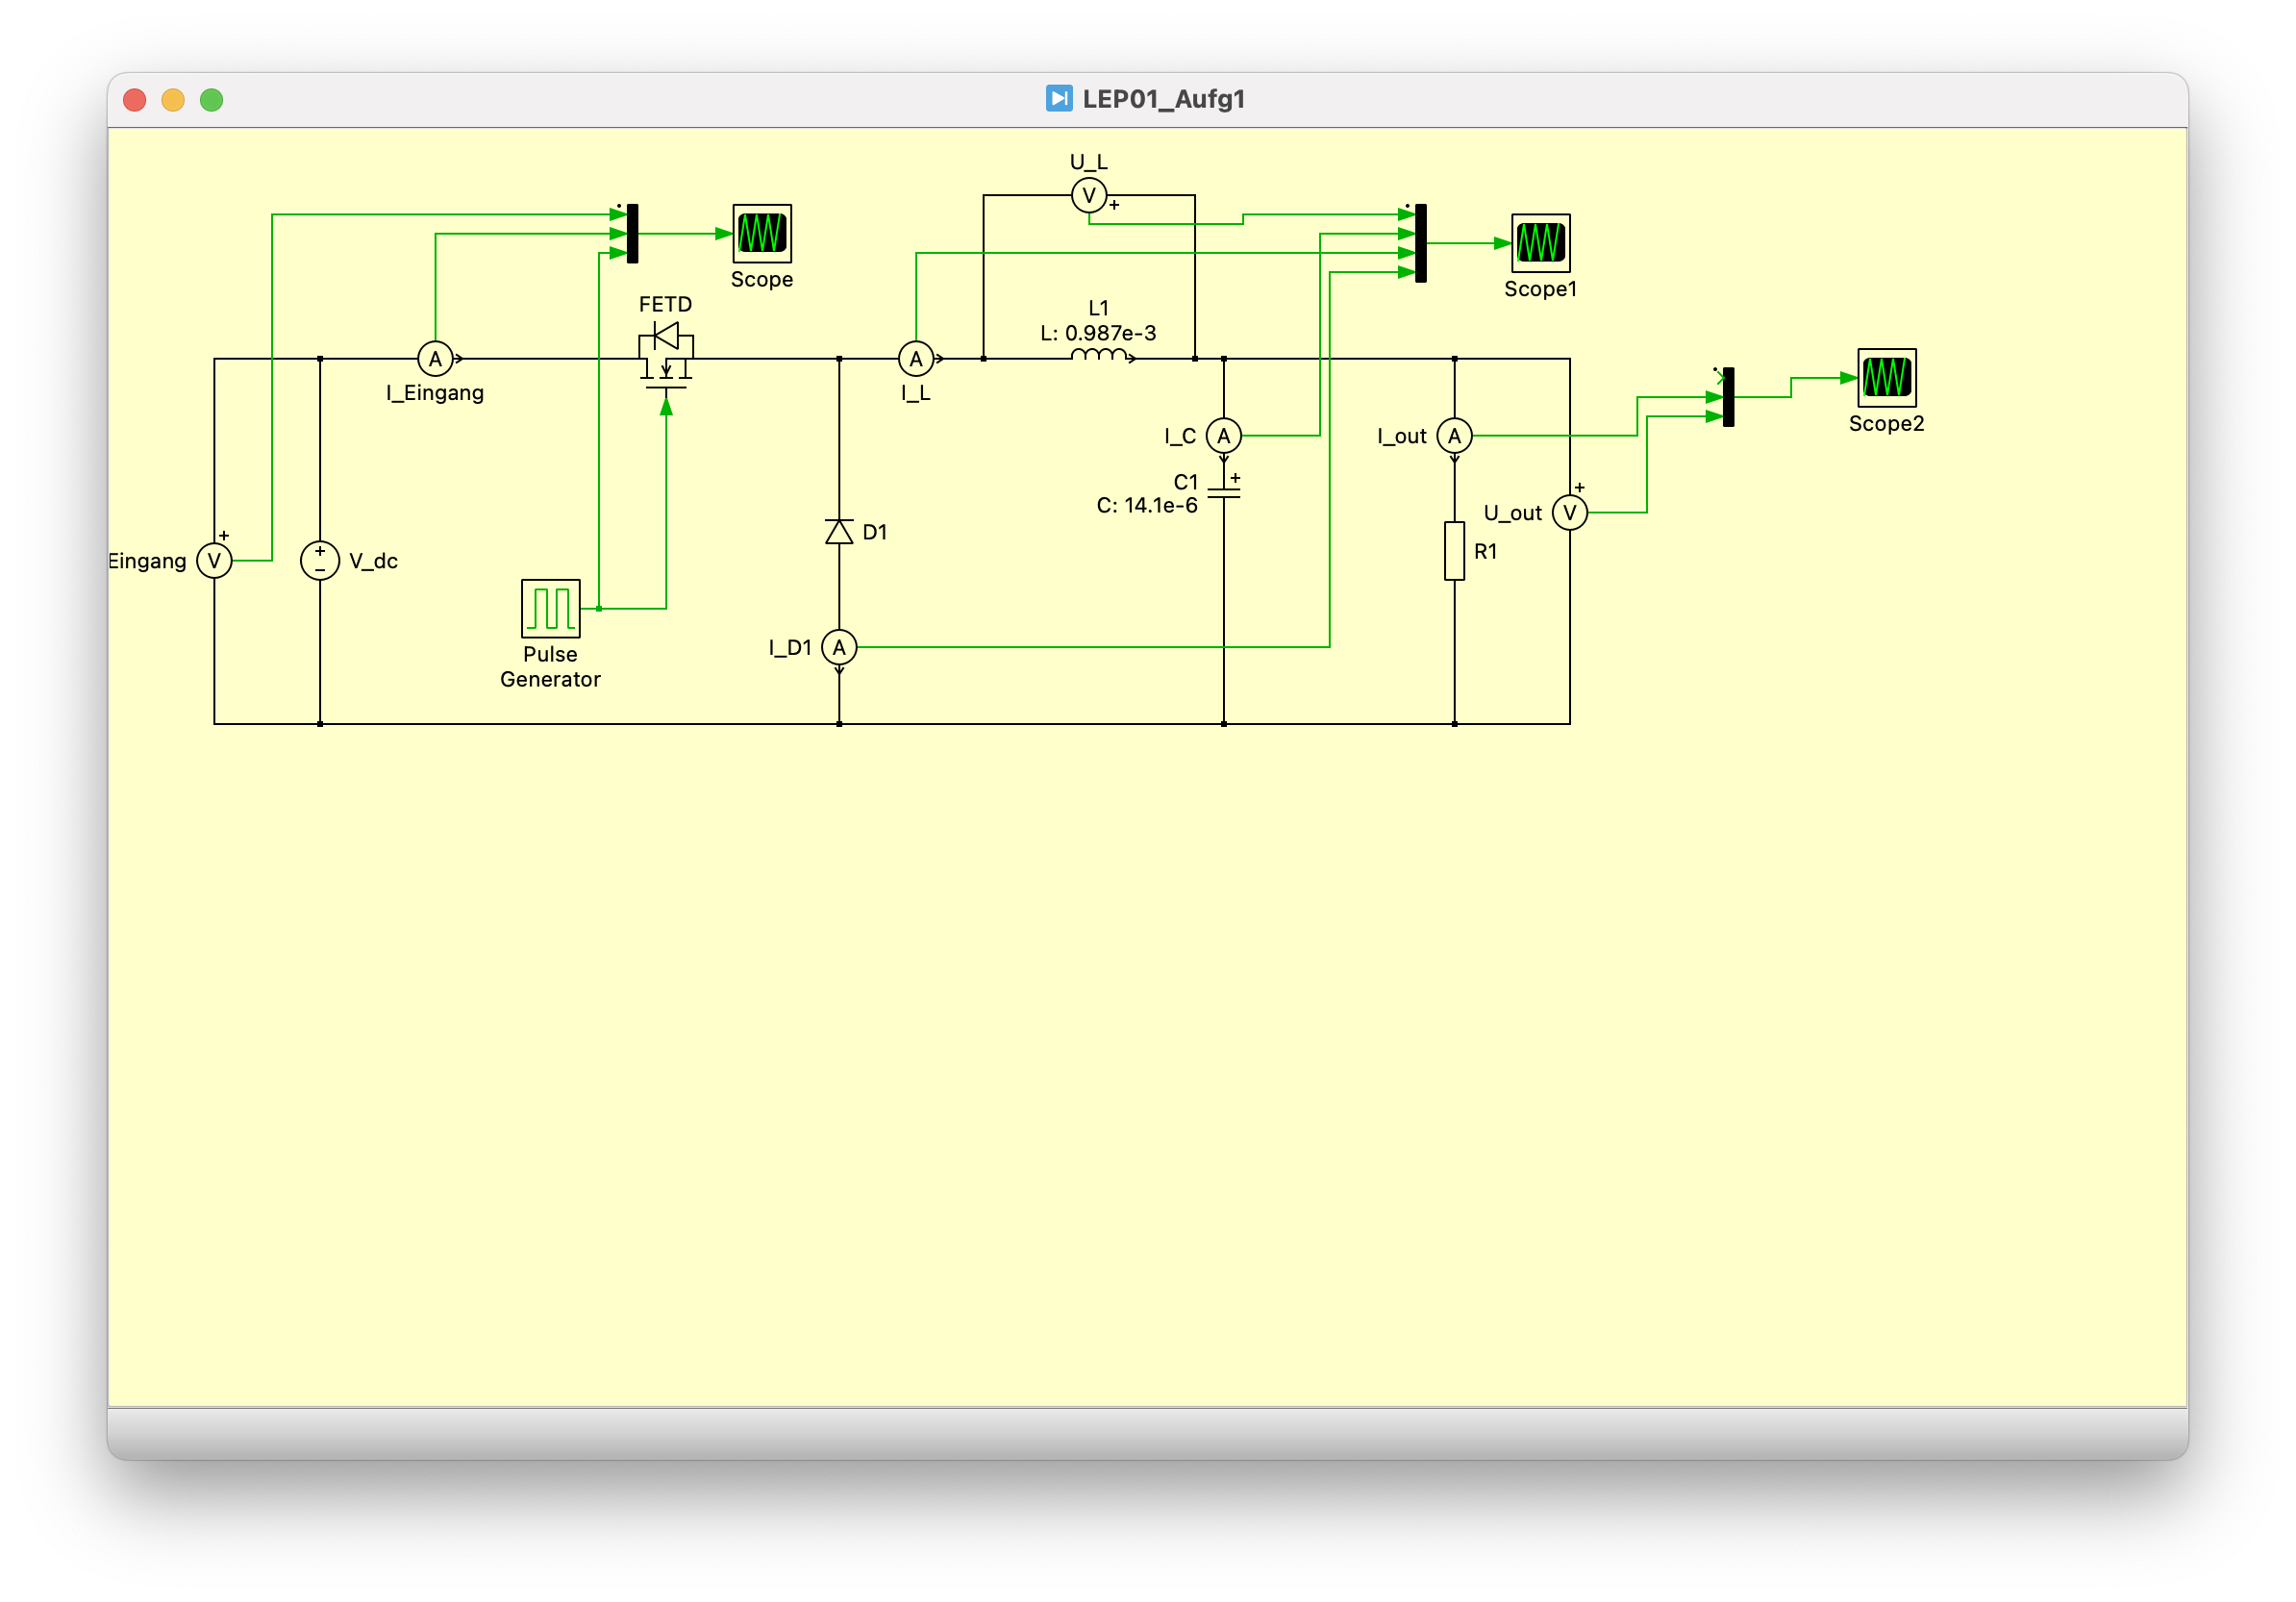
\includegraphics[width=0.95\textwidth]{assets/img/aufg1_aufbau.png}
  \end{center}
  \caption{Der Aufbau der Schaltung mit Messstellen}
  \label{fig:aufg1_aufbau}
\end{figure}

Bei der Simulation wird die Eingangsspannung auf $U_e = 160V$ und der PWM-Generator auf $0,45$ Duty Cycle gestellt. (siehe )

\begin{figure}
  \begin{center}
    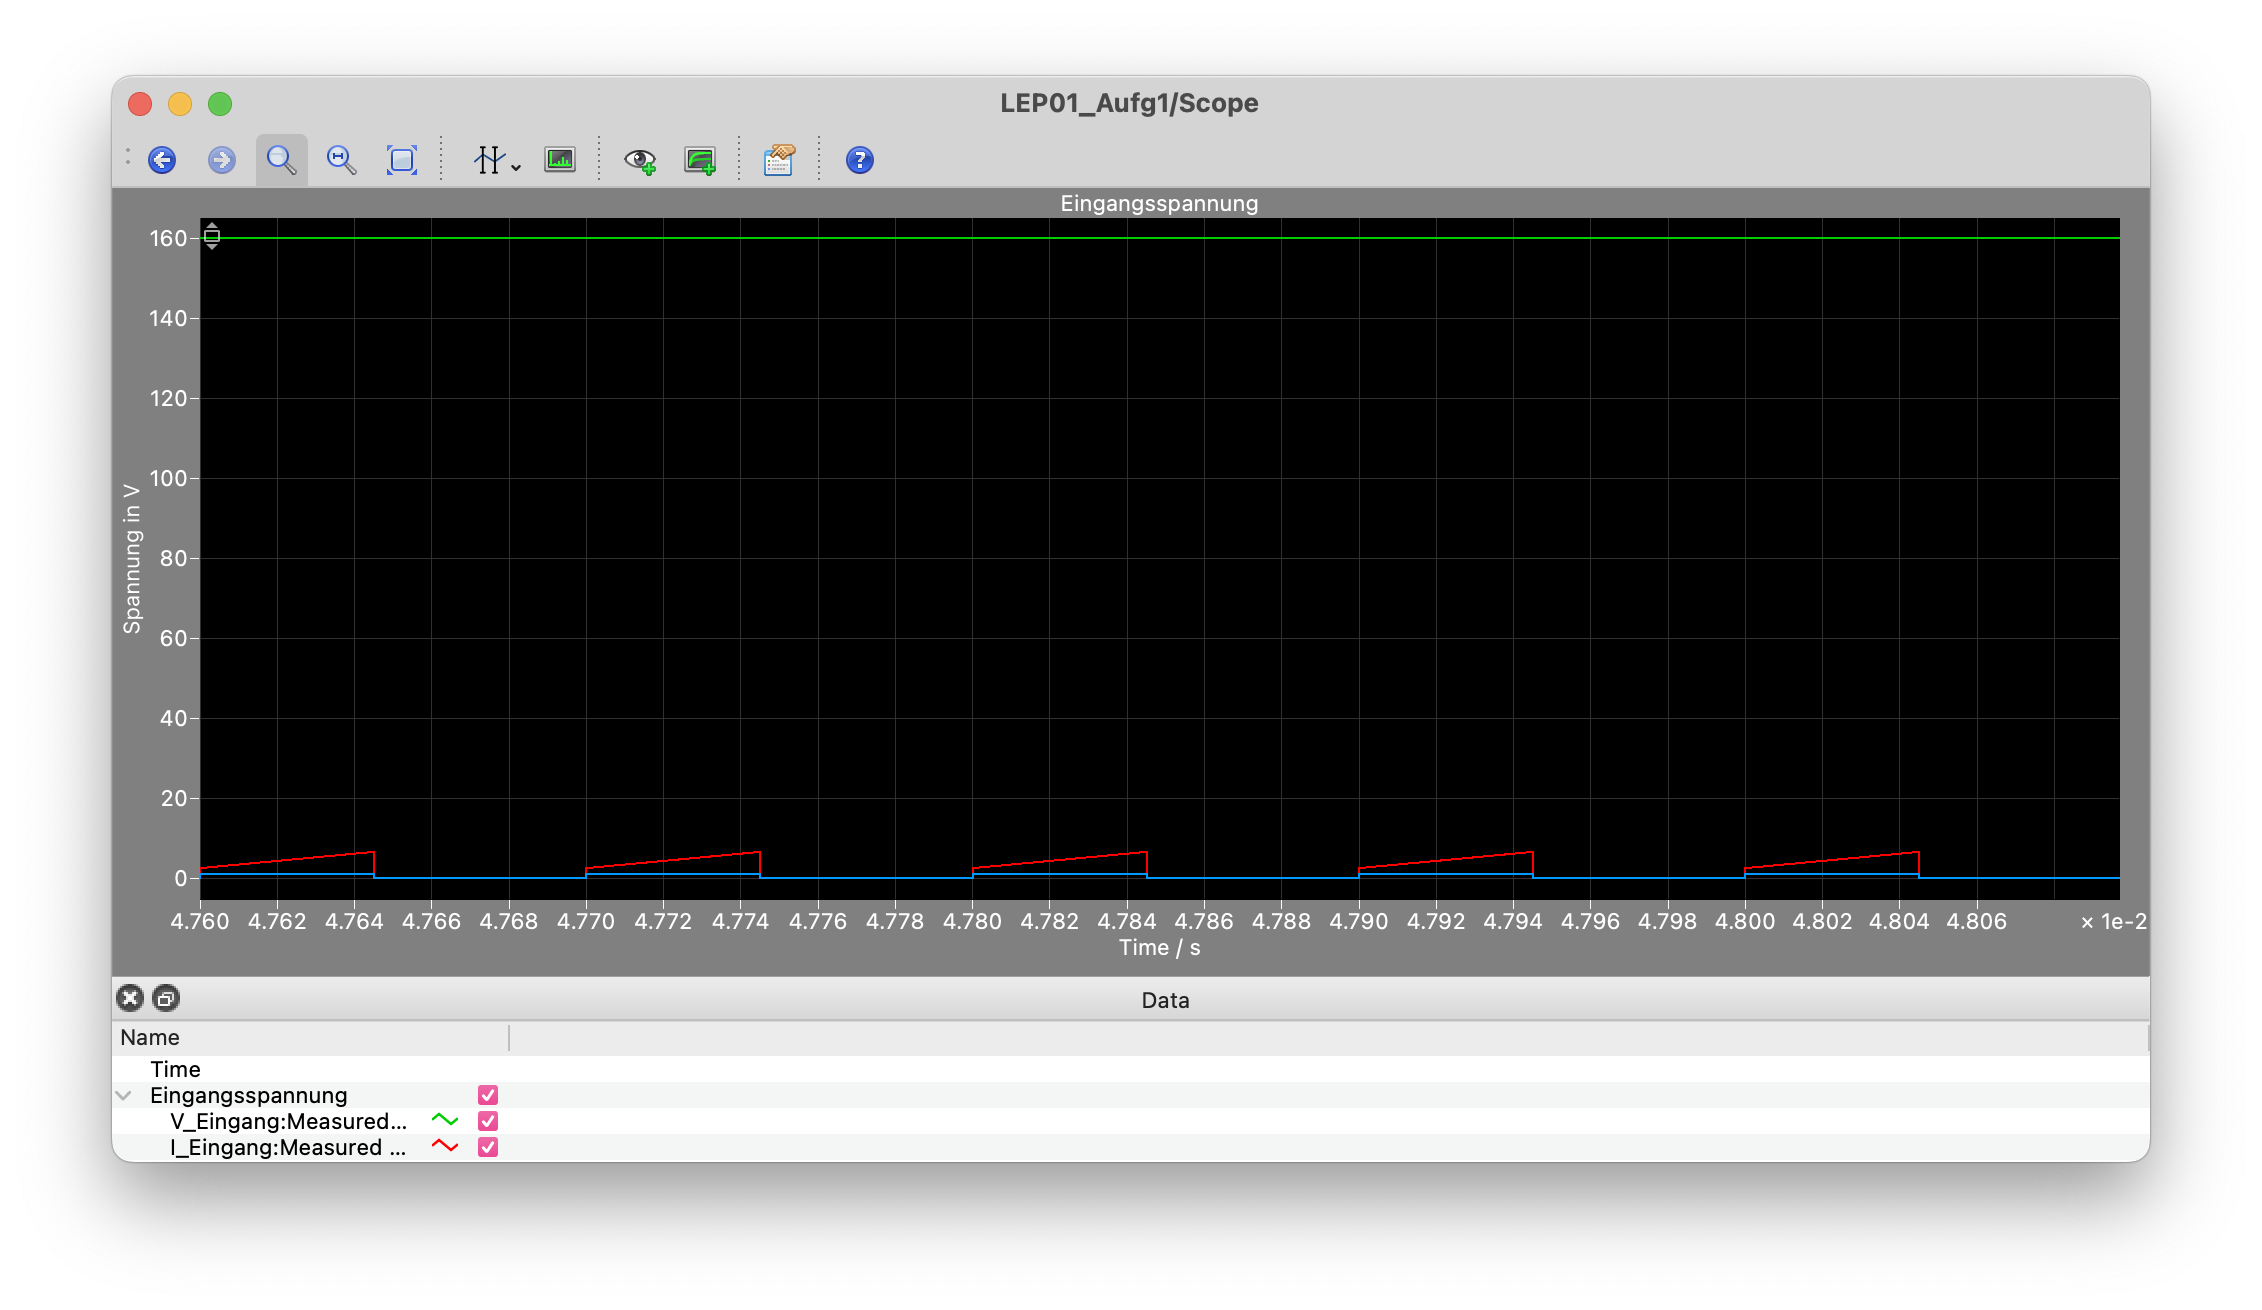
\includegraphics[width=0.95\textwidth]{./assets/img/aufg1_eingang.png}
  \end{center}
  \caption{Die Eingangstraces für den Tiefsetzsteller. $U_e$ (grün), $PWM$ (blau), $I_e$ (rot)}
  \label{fig:aufg1_eingang}
\end{figure}

Im Tiefsetzsteller werden nun die folgenden Traces aufgenommen:

\begin{figure}
  \begin{center}
    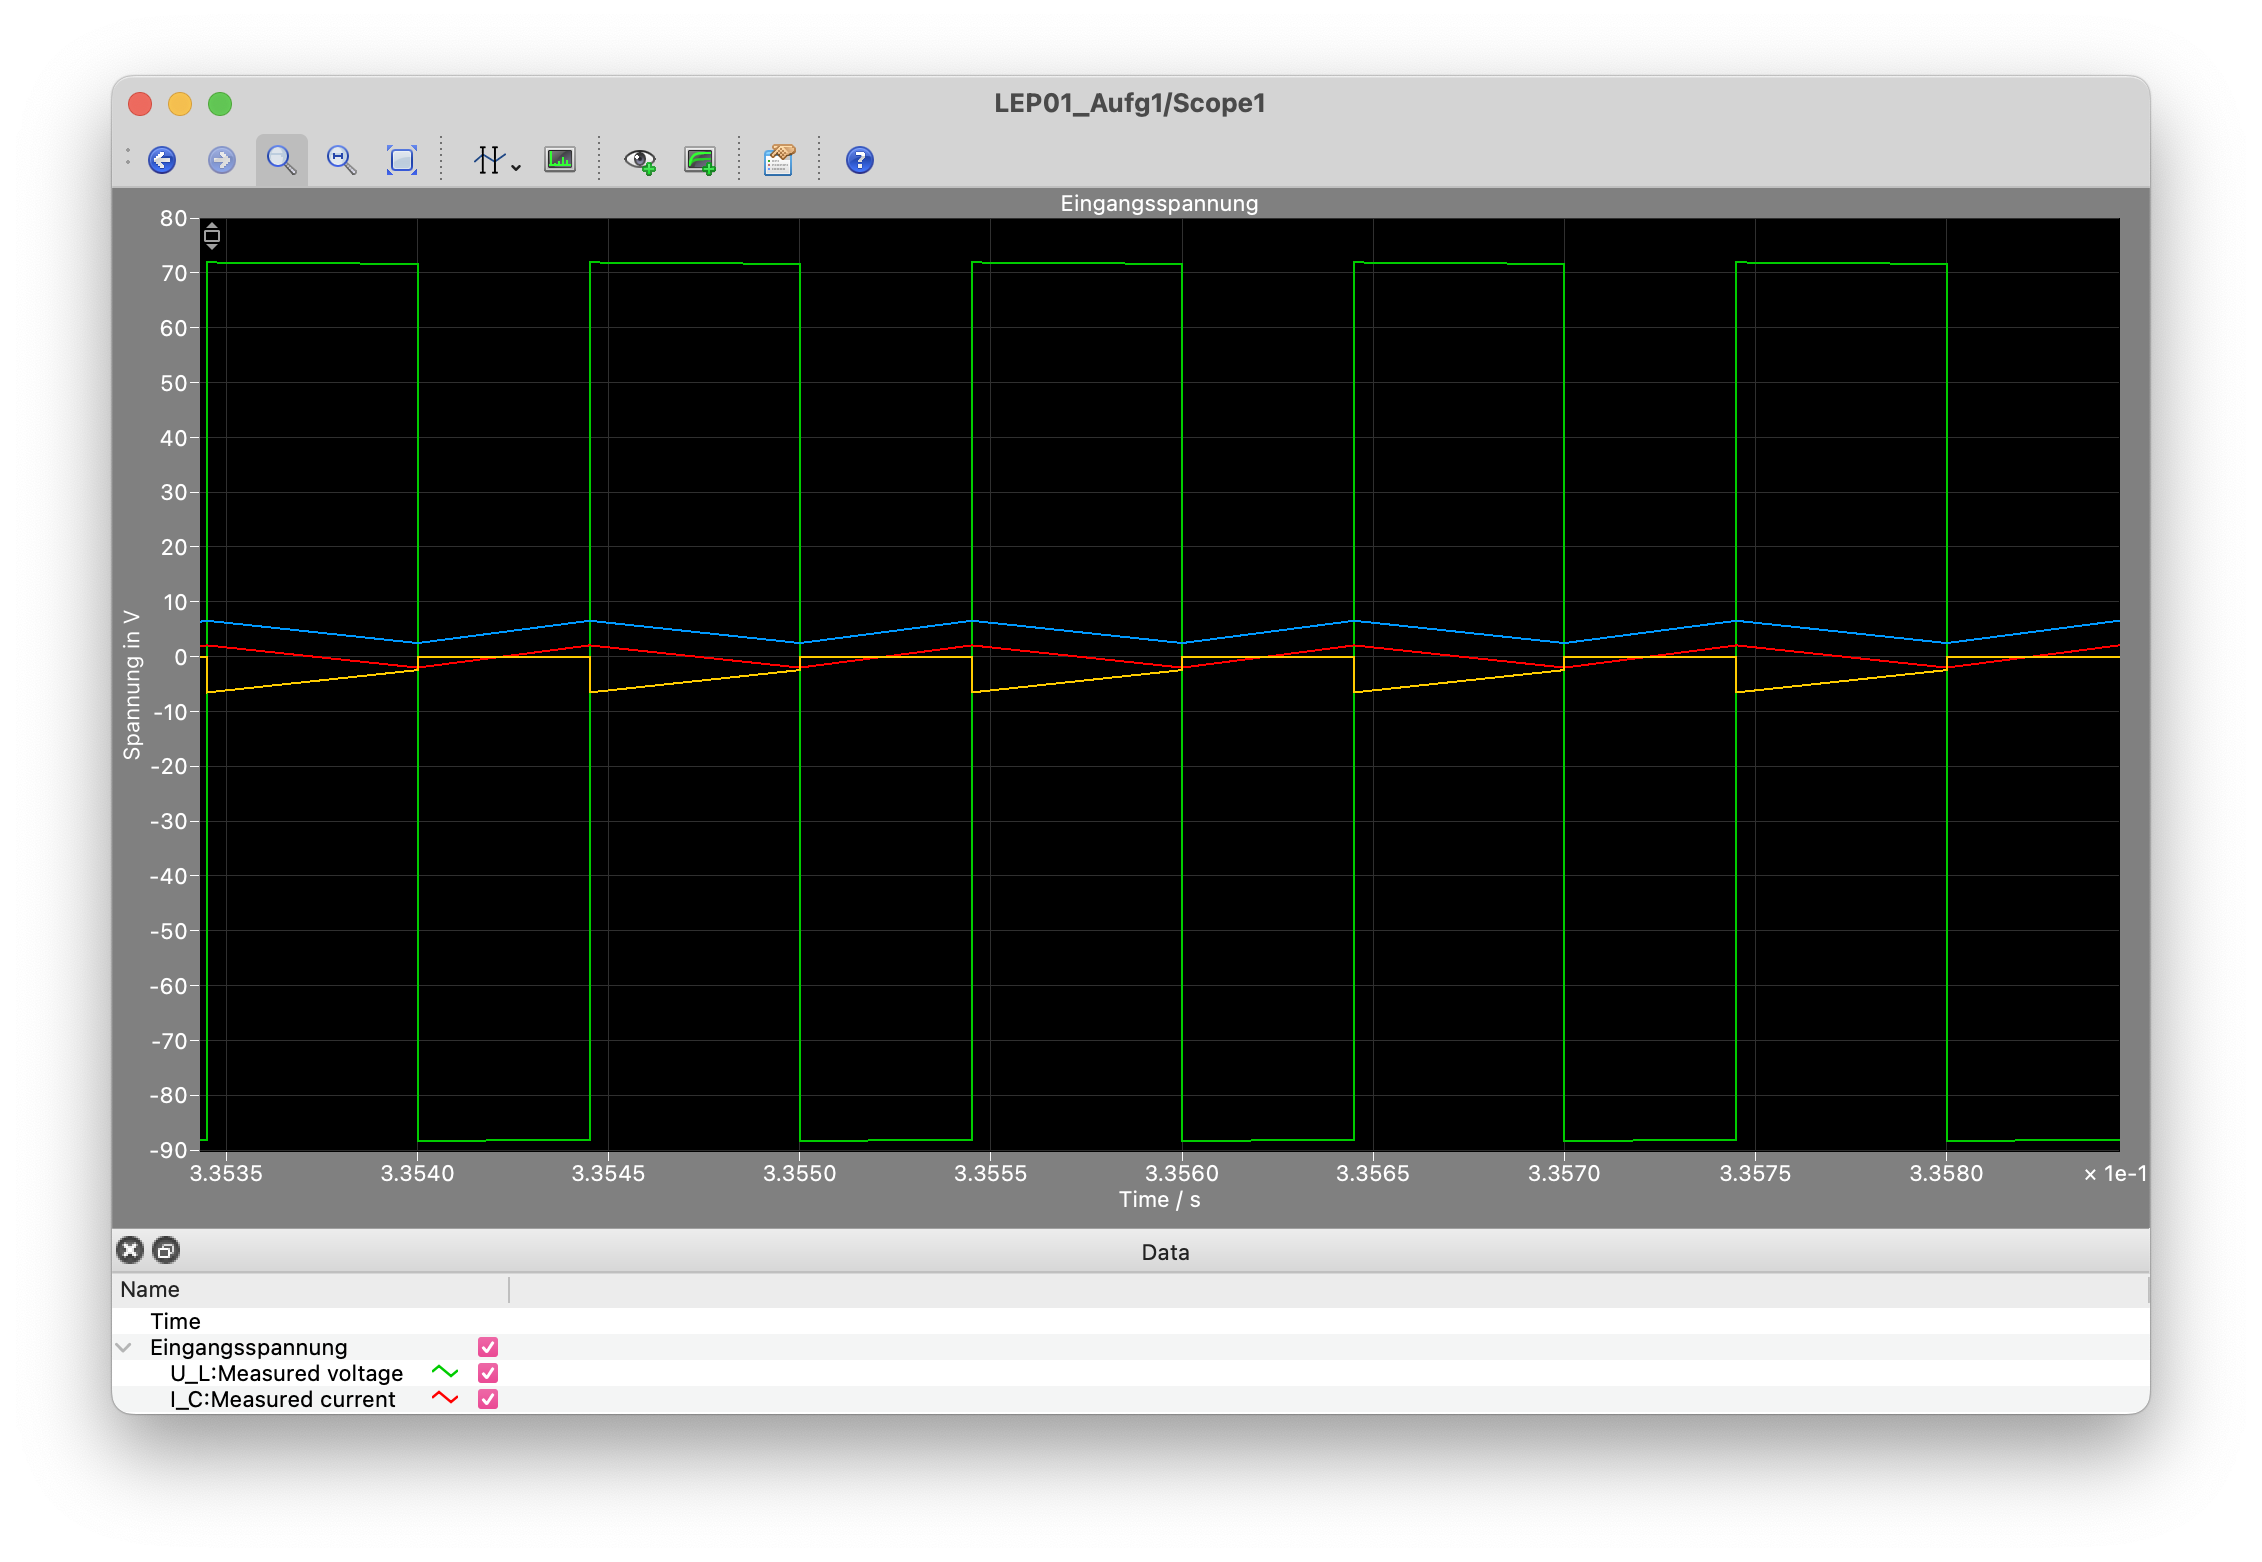
\includegraphics[width=0.95\textwidth]{assets/img/aufg1_strecke.png}
  \end{center}
  \caption{Die Tiefsetzsteller-Strecke mit den Strömen und Spannungen über die Bauteile. $I_C$ (rot), $I_L$ (blau), $I_D$ (gelb), $U_L$ (grün)}
  \label{fig:aufg1_strecke}
\end{figure}

Der Ausgang des Tiefsetzstellers kann nun über die folgenden Traces beschrieben werden:

\begin{figure}
  \begin{center}
    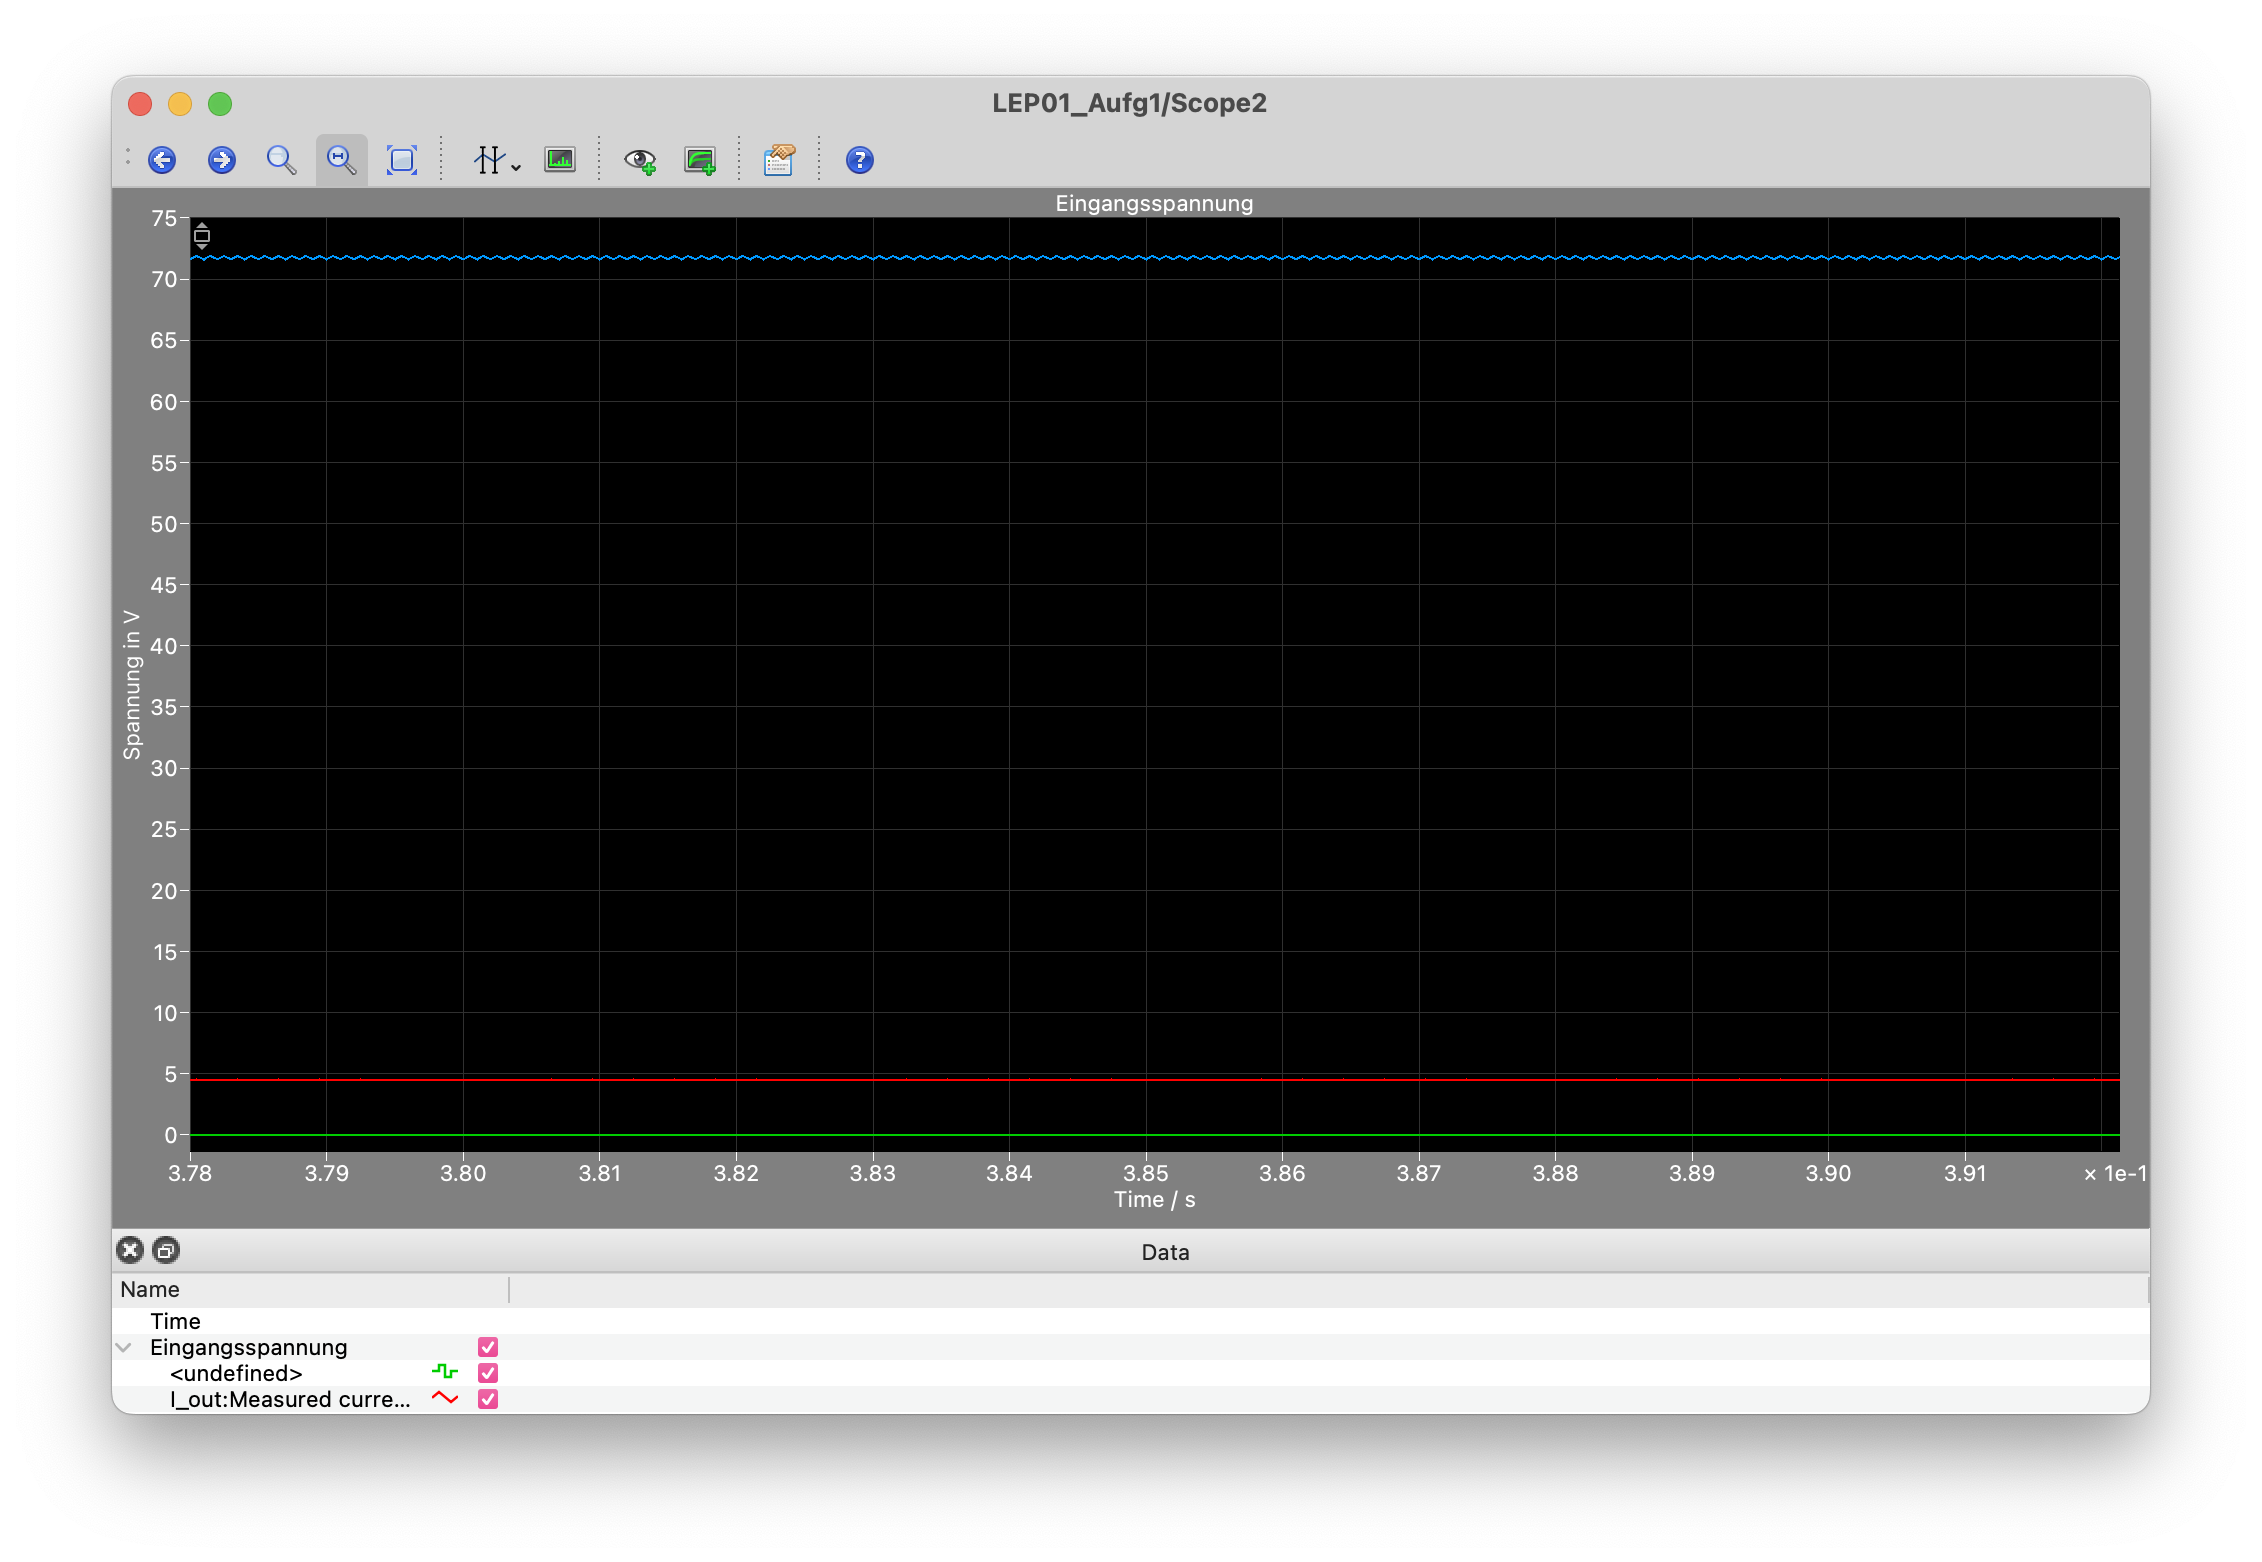
\includegraphics[width=0.95\textwidth]{assets/img/aufg1_ausgang.png}
  \end{center}
  \caption{Der Ausgang des Tiefsetzstellers mit der Ausgangsspannung und dem Ausgangsstrom. $I_a$ (rot), $U_a$ (blau)}
  \label{fig:aufg1_ausgang}
\end{figure}

\subsection{Auswertung}

Es ist erkennbar, dass die geforderten Ausgangswerte mit den simulierten Werten in dieser Aufgabe übereinstimmen. Bei einer Eingangsspannung $U_e = 160V$ kann eine Batterie mit einer möglichen Ladespannung $U_a = 72V$ über den Tiefsetzsteller geladen werden. Der maximale Lastabfall wird nicht überschritten. Deutlich erkennbar ist das Verhalten des Tiefsetzstellers im Zusammenhang mit dem PWM-Signal funktioniert und eine kleinere Spannung erzeugt werden kann, die über den Duty Cycle des PWM-Generators steuerbar ist. 

\section{Aufgabe 2}

In Aufgabe 2 wird nun ein eigner PWM-Generator mit der PLECS-Software aufgebaut. Dieser steuert dann einen Wechselrichter. Beide Schaltungen sollen analysiert und ausgewertet werden.

\subsection{Aufbau und Simulation}

Zunächst wird der PWM-Generator aufgebaut: 

\begin{figure}
  \begin{center}
  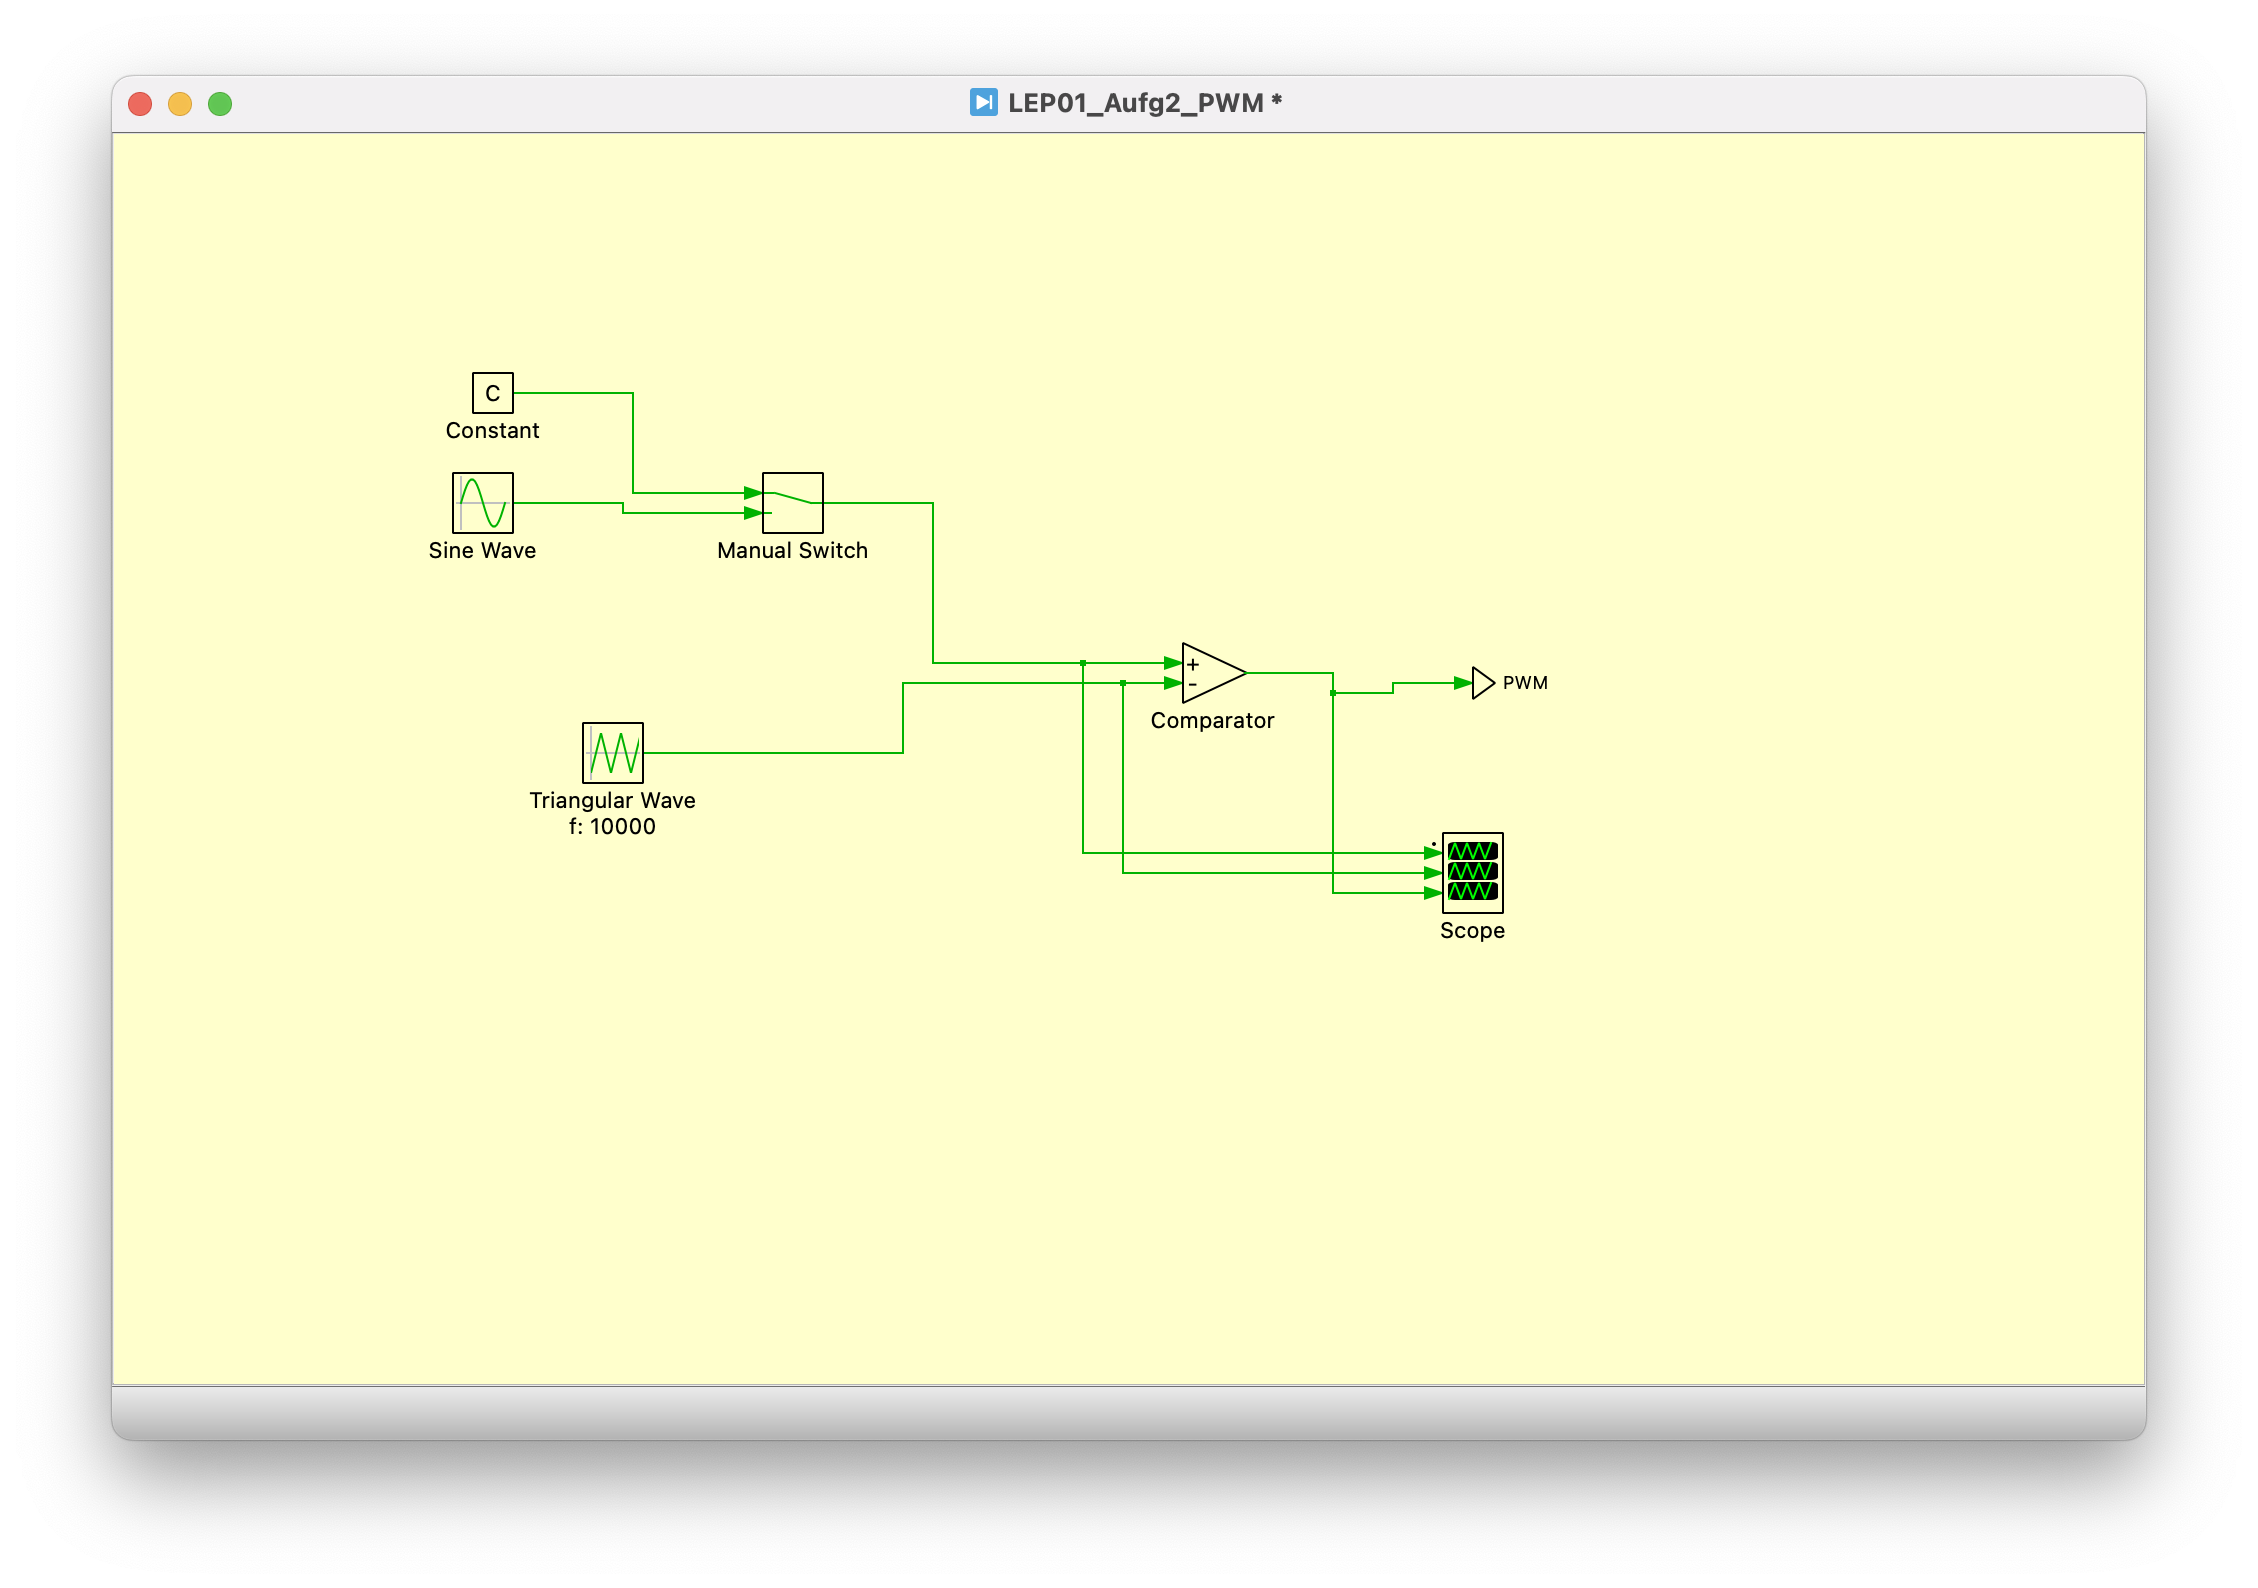
\includegraphics[width=0.95\textwidth]{assets/img/aufg2_aufbau_pwm.png}
  \end{center}
  \caption{Der Aufbau des PWM-Generators}
  \label{fig:aufg2_aufbau_pwm}
\end{figure}


Wichtig zu bemerken ist hier die Möglichkeit, den PWM-Generator zwischen einem konstanten Duty Cycle und eines Sinus-Signals ($0\% - 100\%$, $f=50Hz$) umzuschalten. Im Betrieb mit einem konstanten Duty Cycle entspricht dieser PWM-Generator dem PWM-Generator, der auch in Aufgabe 1 verwendet wurde. Eine dynamische Änderung des Duty Cycles mittels des Sinus-Signales wird im folgenden untersucht.

\begin{figure}[h]
  \begin{center}
    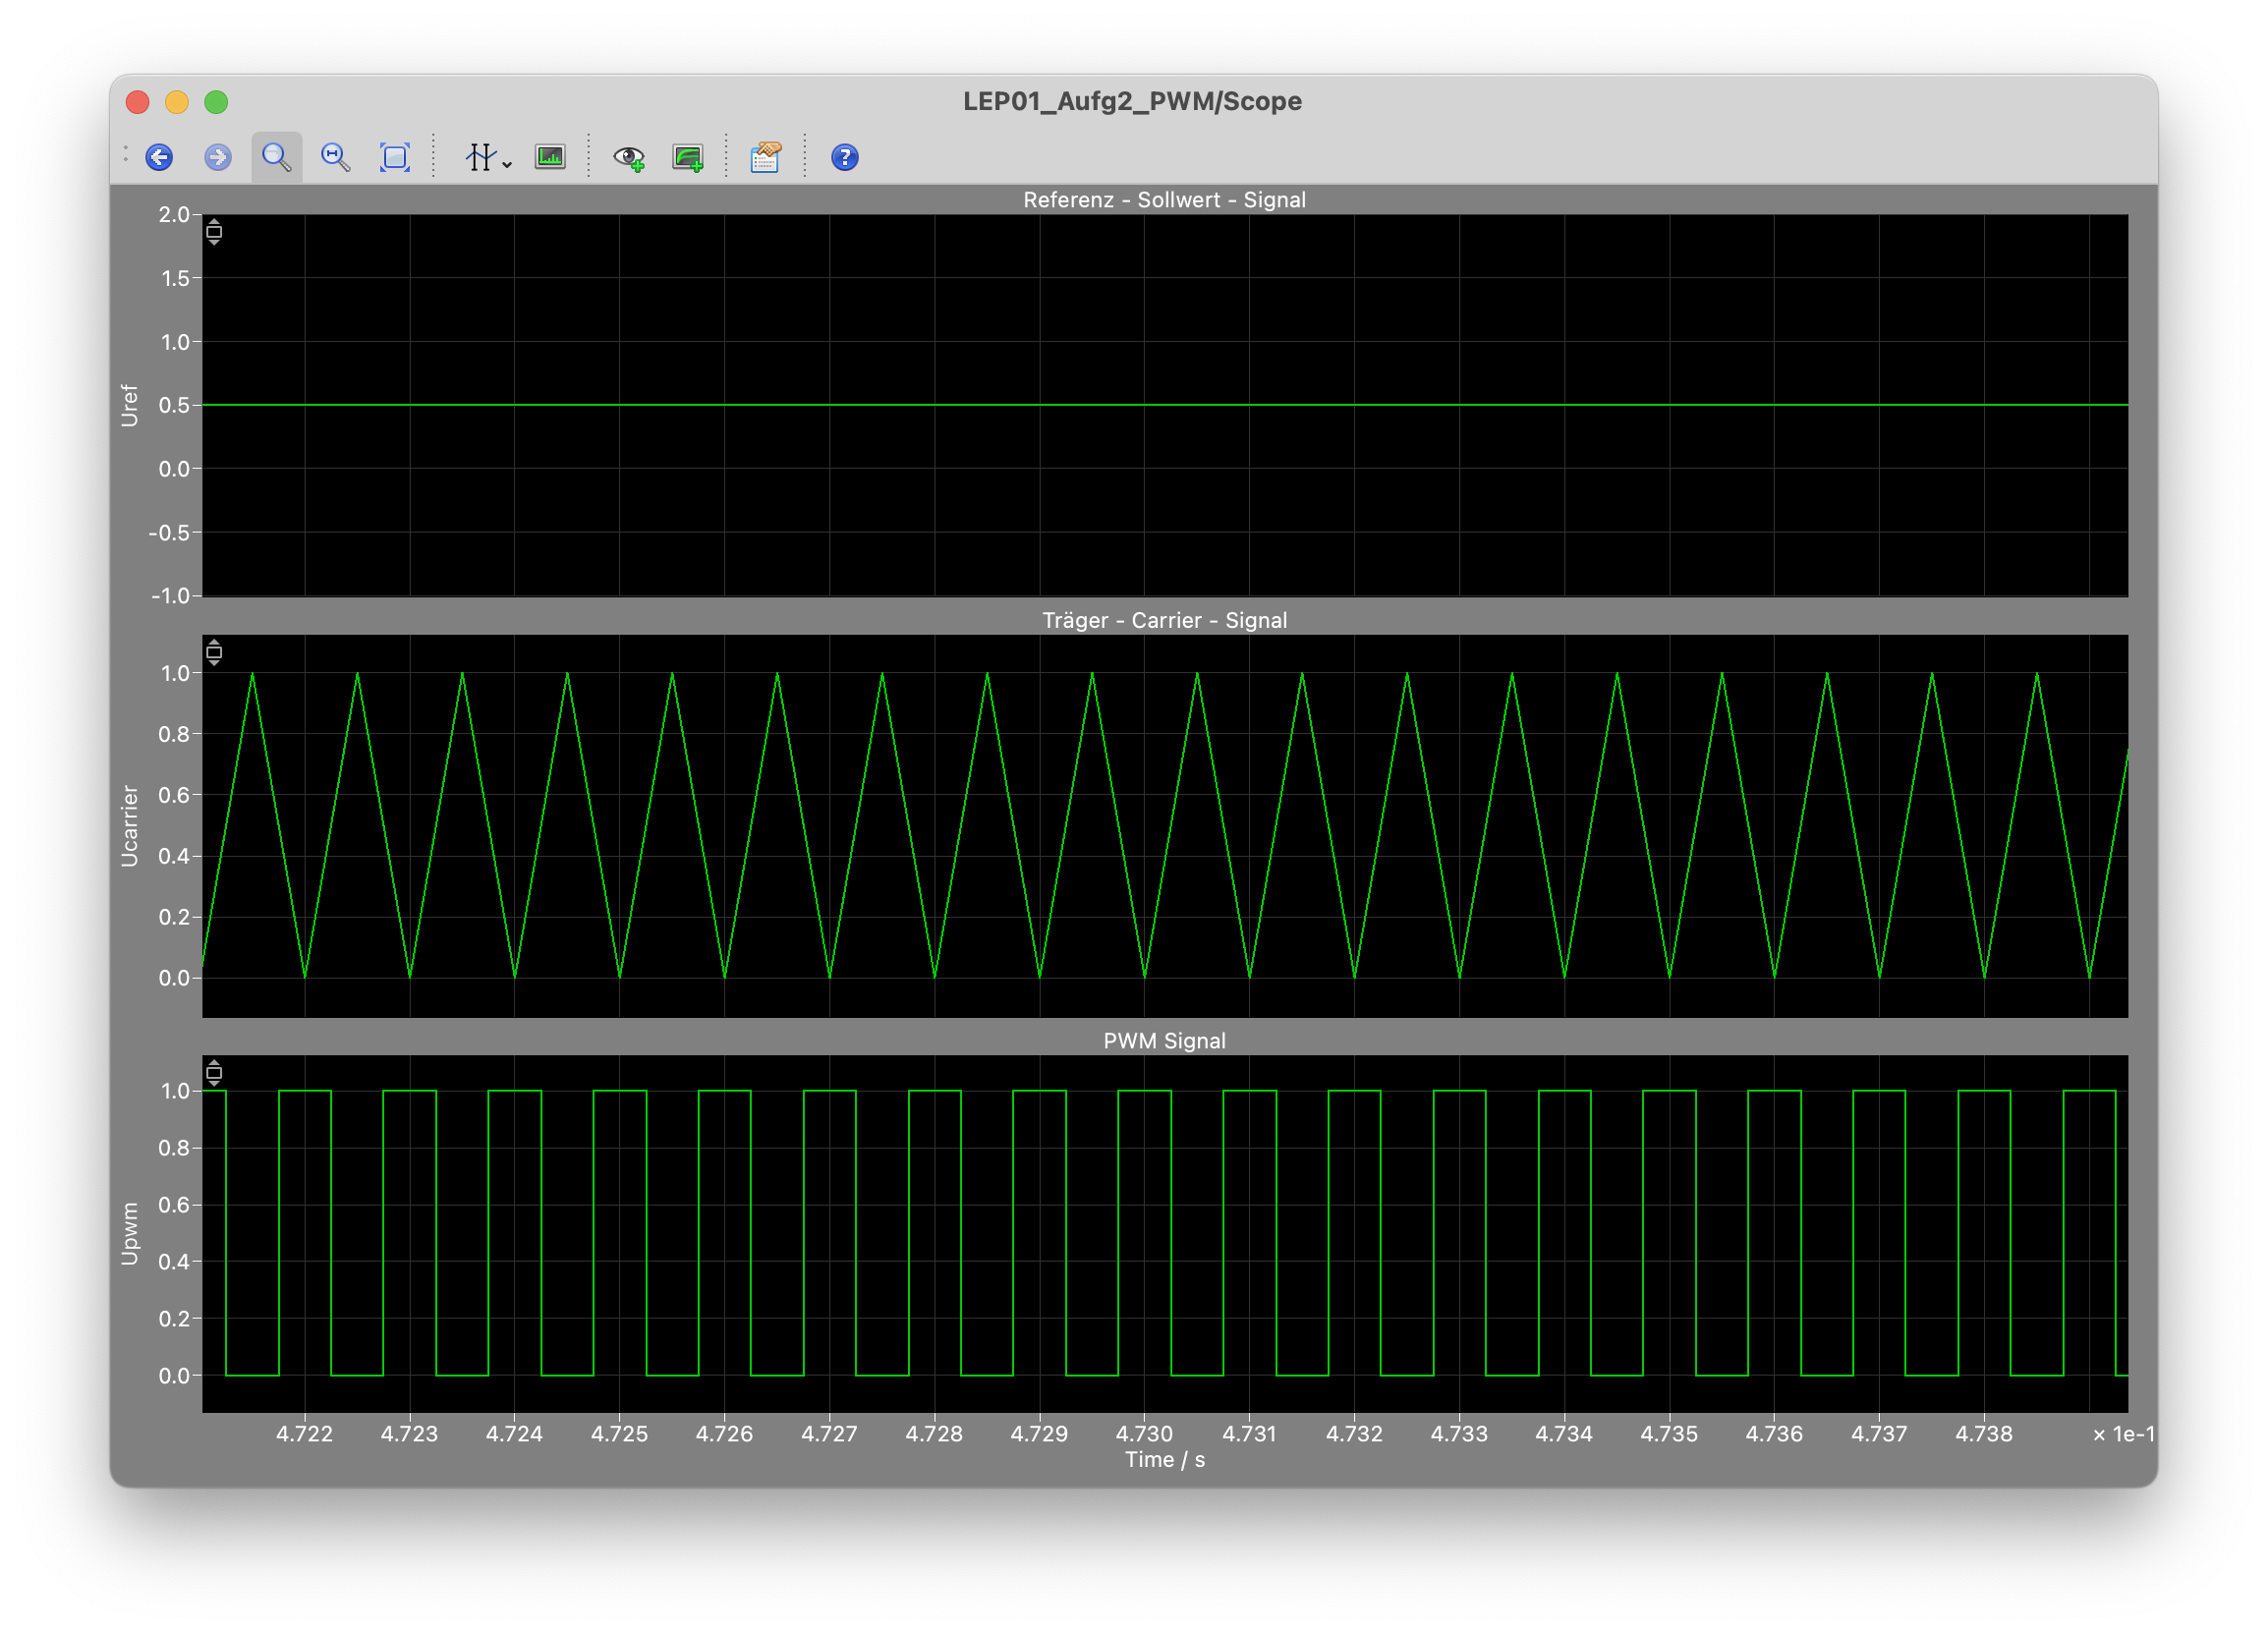
\includegraphics[width=0.95\textwidth]{assets/img/aufg2_pwm_c.png}
  \end{center}
  \caption{Das PWM-Signal durch ein konstantes Gate-Signal gesteuert. Duty Cycle bei $D=0.5$}
  \label{fig:aufg2_pwm_c}
\end{figure}

\begin{figure}[h]
  \begin{center}
    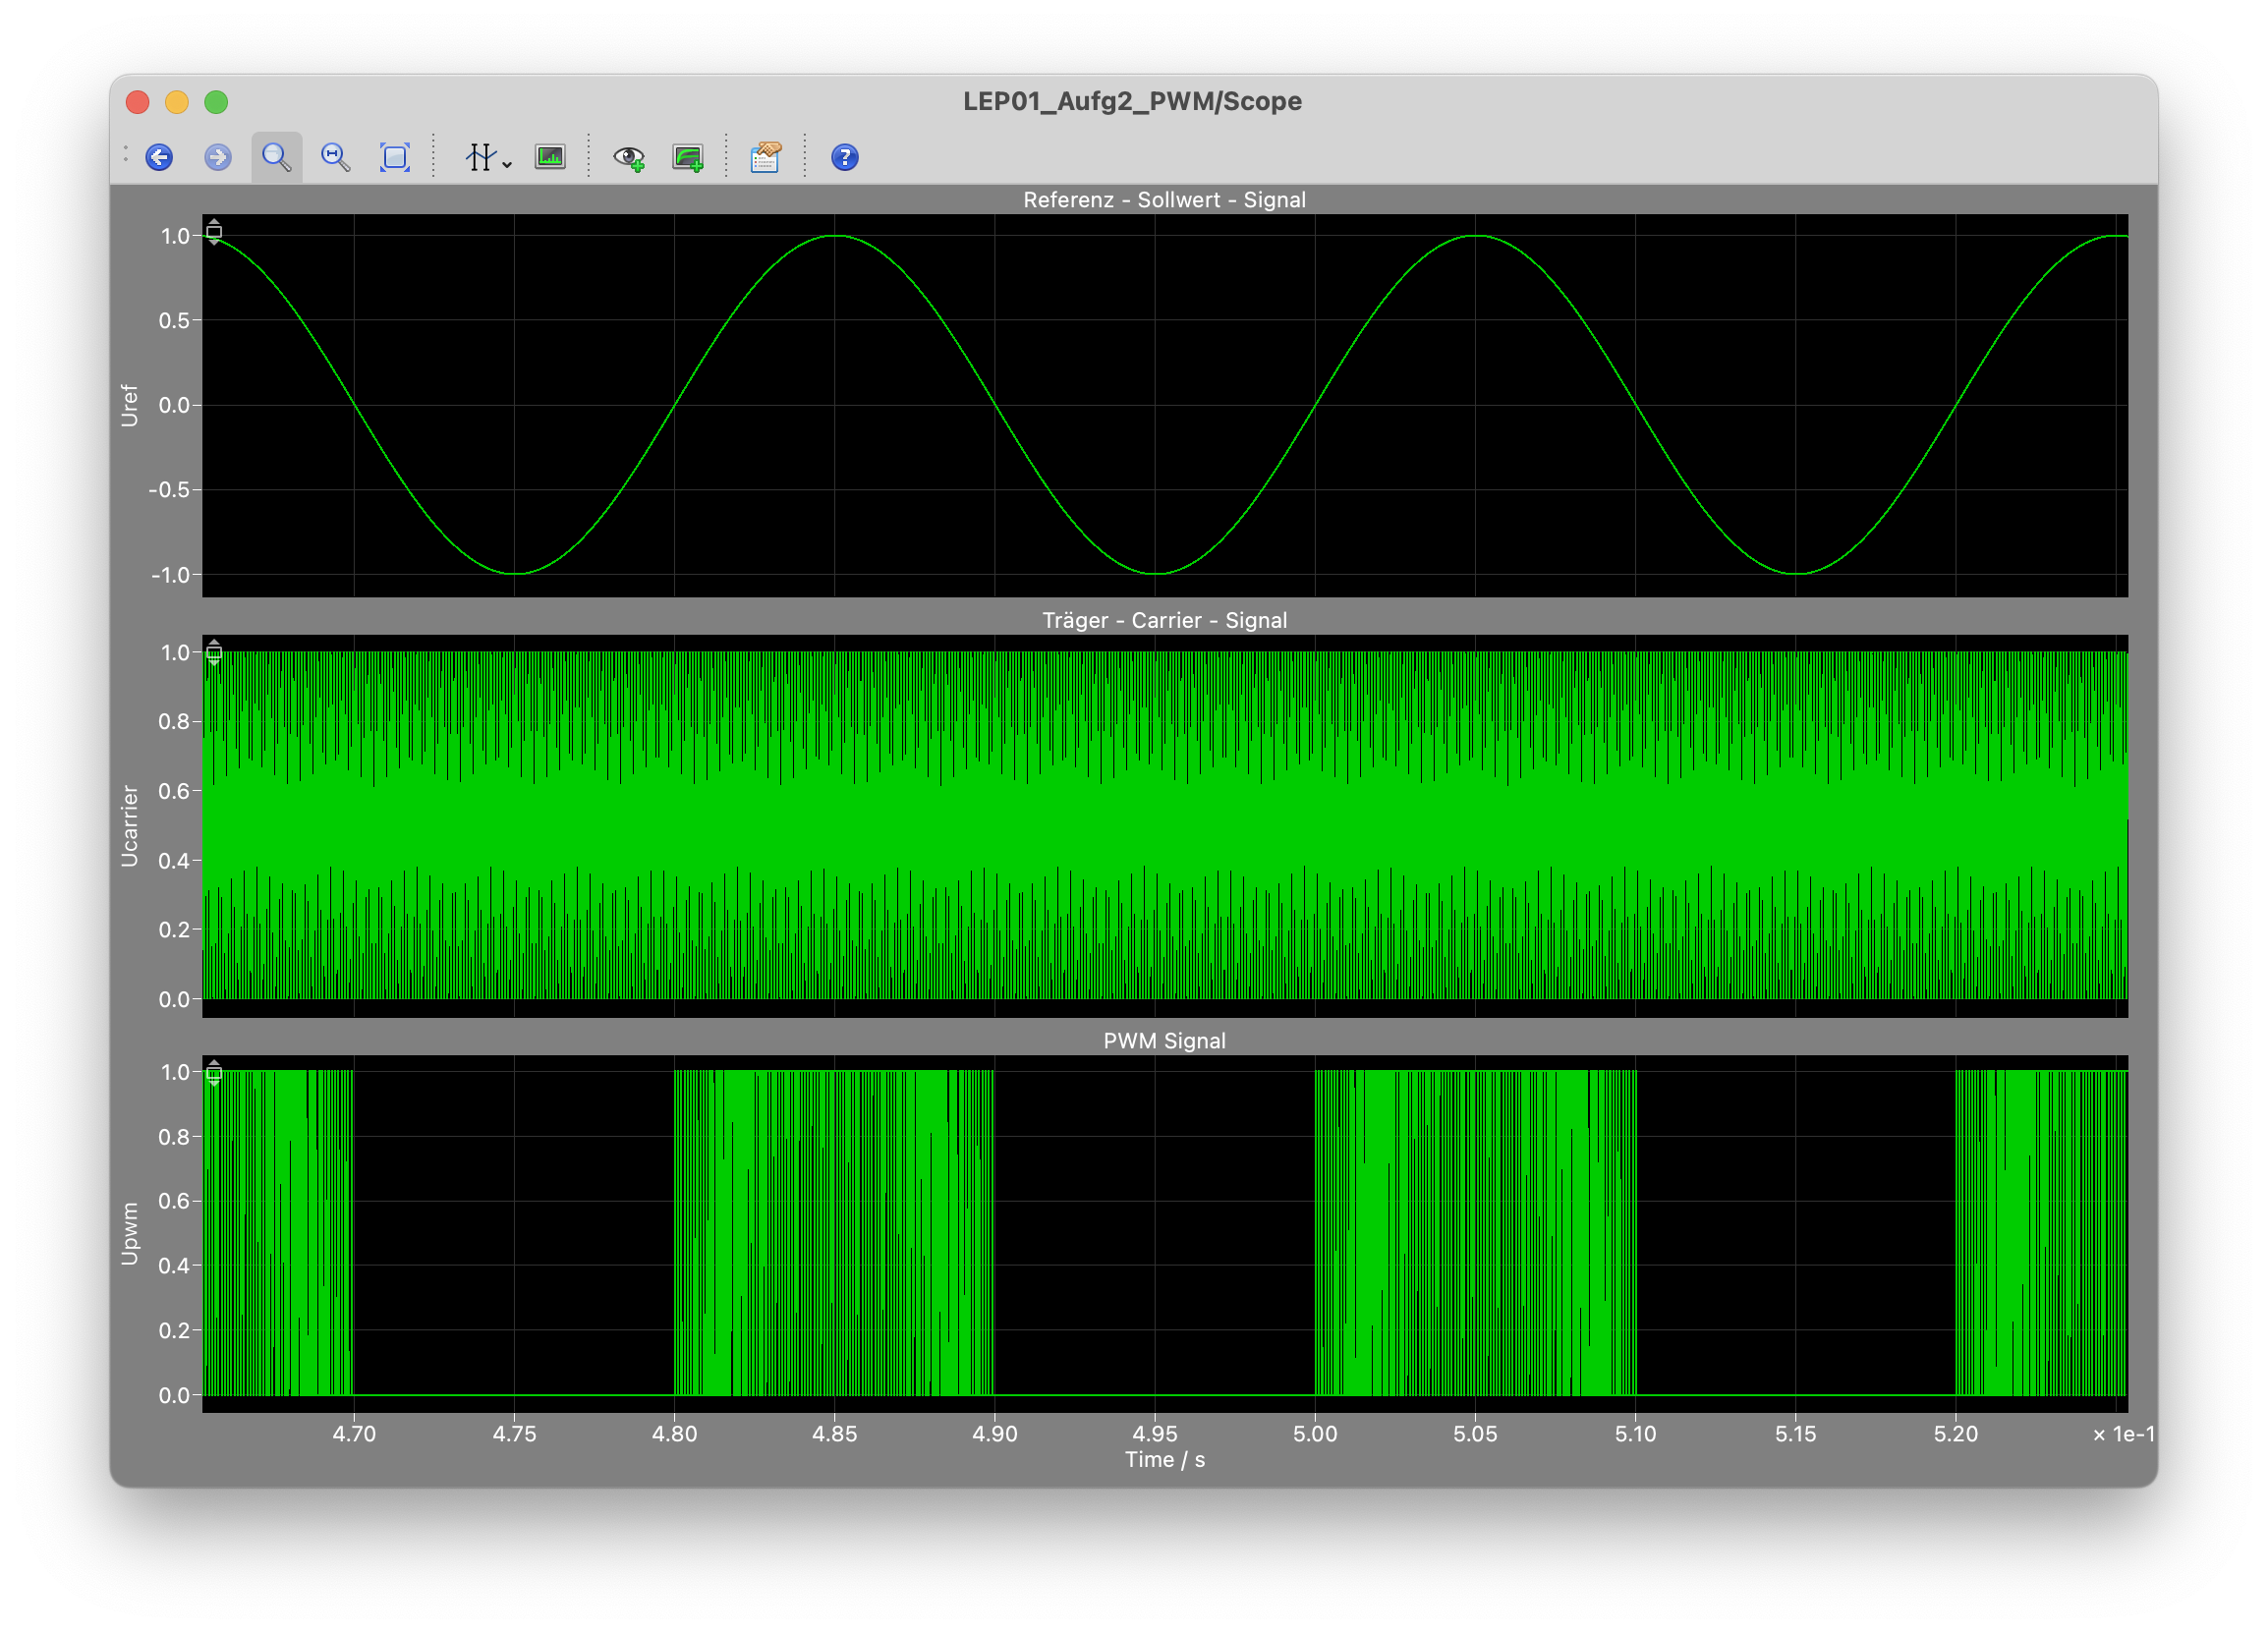
\includegraphics[width=0.95\textwidth]{assets/img/aufg2_pwm_sin.png}
  \end{center}
  \caption{Das PWM-Signal durch einen Sinus-Oszillator gesteuert (50Hz)}
  \label{fig:aufg2_pwm_sin}
\end{figure}

In Abbildung ~\ref{fig:aufg2_pwm} ist das PWM-Signal zu erkennen, welches auch in Aufgabe 1 verwendet wurde. Durch ein konstantes Signal am nicht-invertierenden Eingang wird aus dem Sägezahn-Carriersignal ein PWM-Signal, bei dem das Tastverhältnis genau ausgeglichen ist.
In Abbildung~\ref{fig:aufg2_pwm_sin} wird nun die selbe Schaltung mit einem Sinus-Steuersignal gezeigt. Ein Wert unter 0 führt in dieser Schaltung zu einem Ausschalten des Signals, da der OpAmp keinen Grund hat, die ungleiche Spannung auszugleichen. Ist das Sinusignal über 0, dann steigt das Tastverhätlnis proportional zu dem Anstieg der Sinuskurve. 

Der Tiefsetzsteller mit entsprechender Brückenschaltung kann in Abbildung~\ref{fig:aufgb2_aufbau} gesehen werden.

\begin{figure}[h]
  \begin{center}
    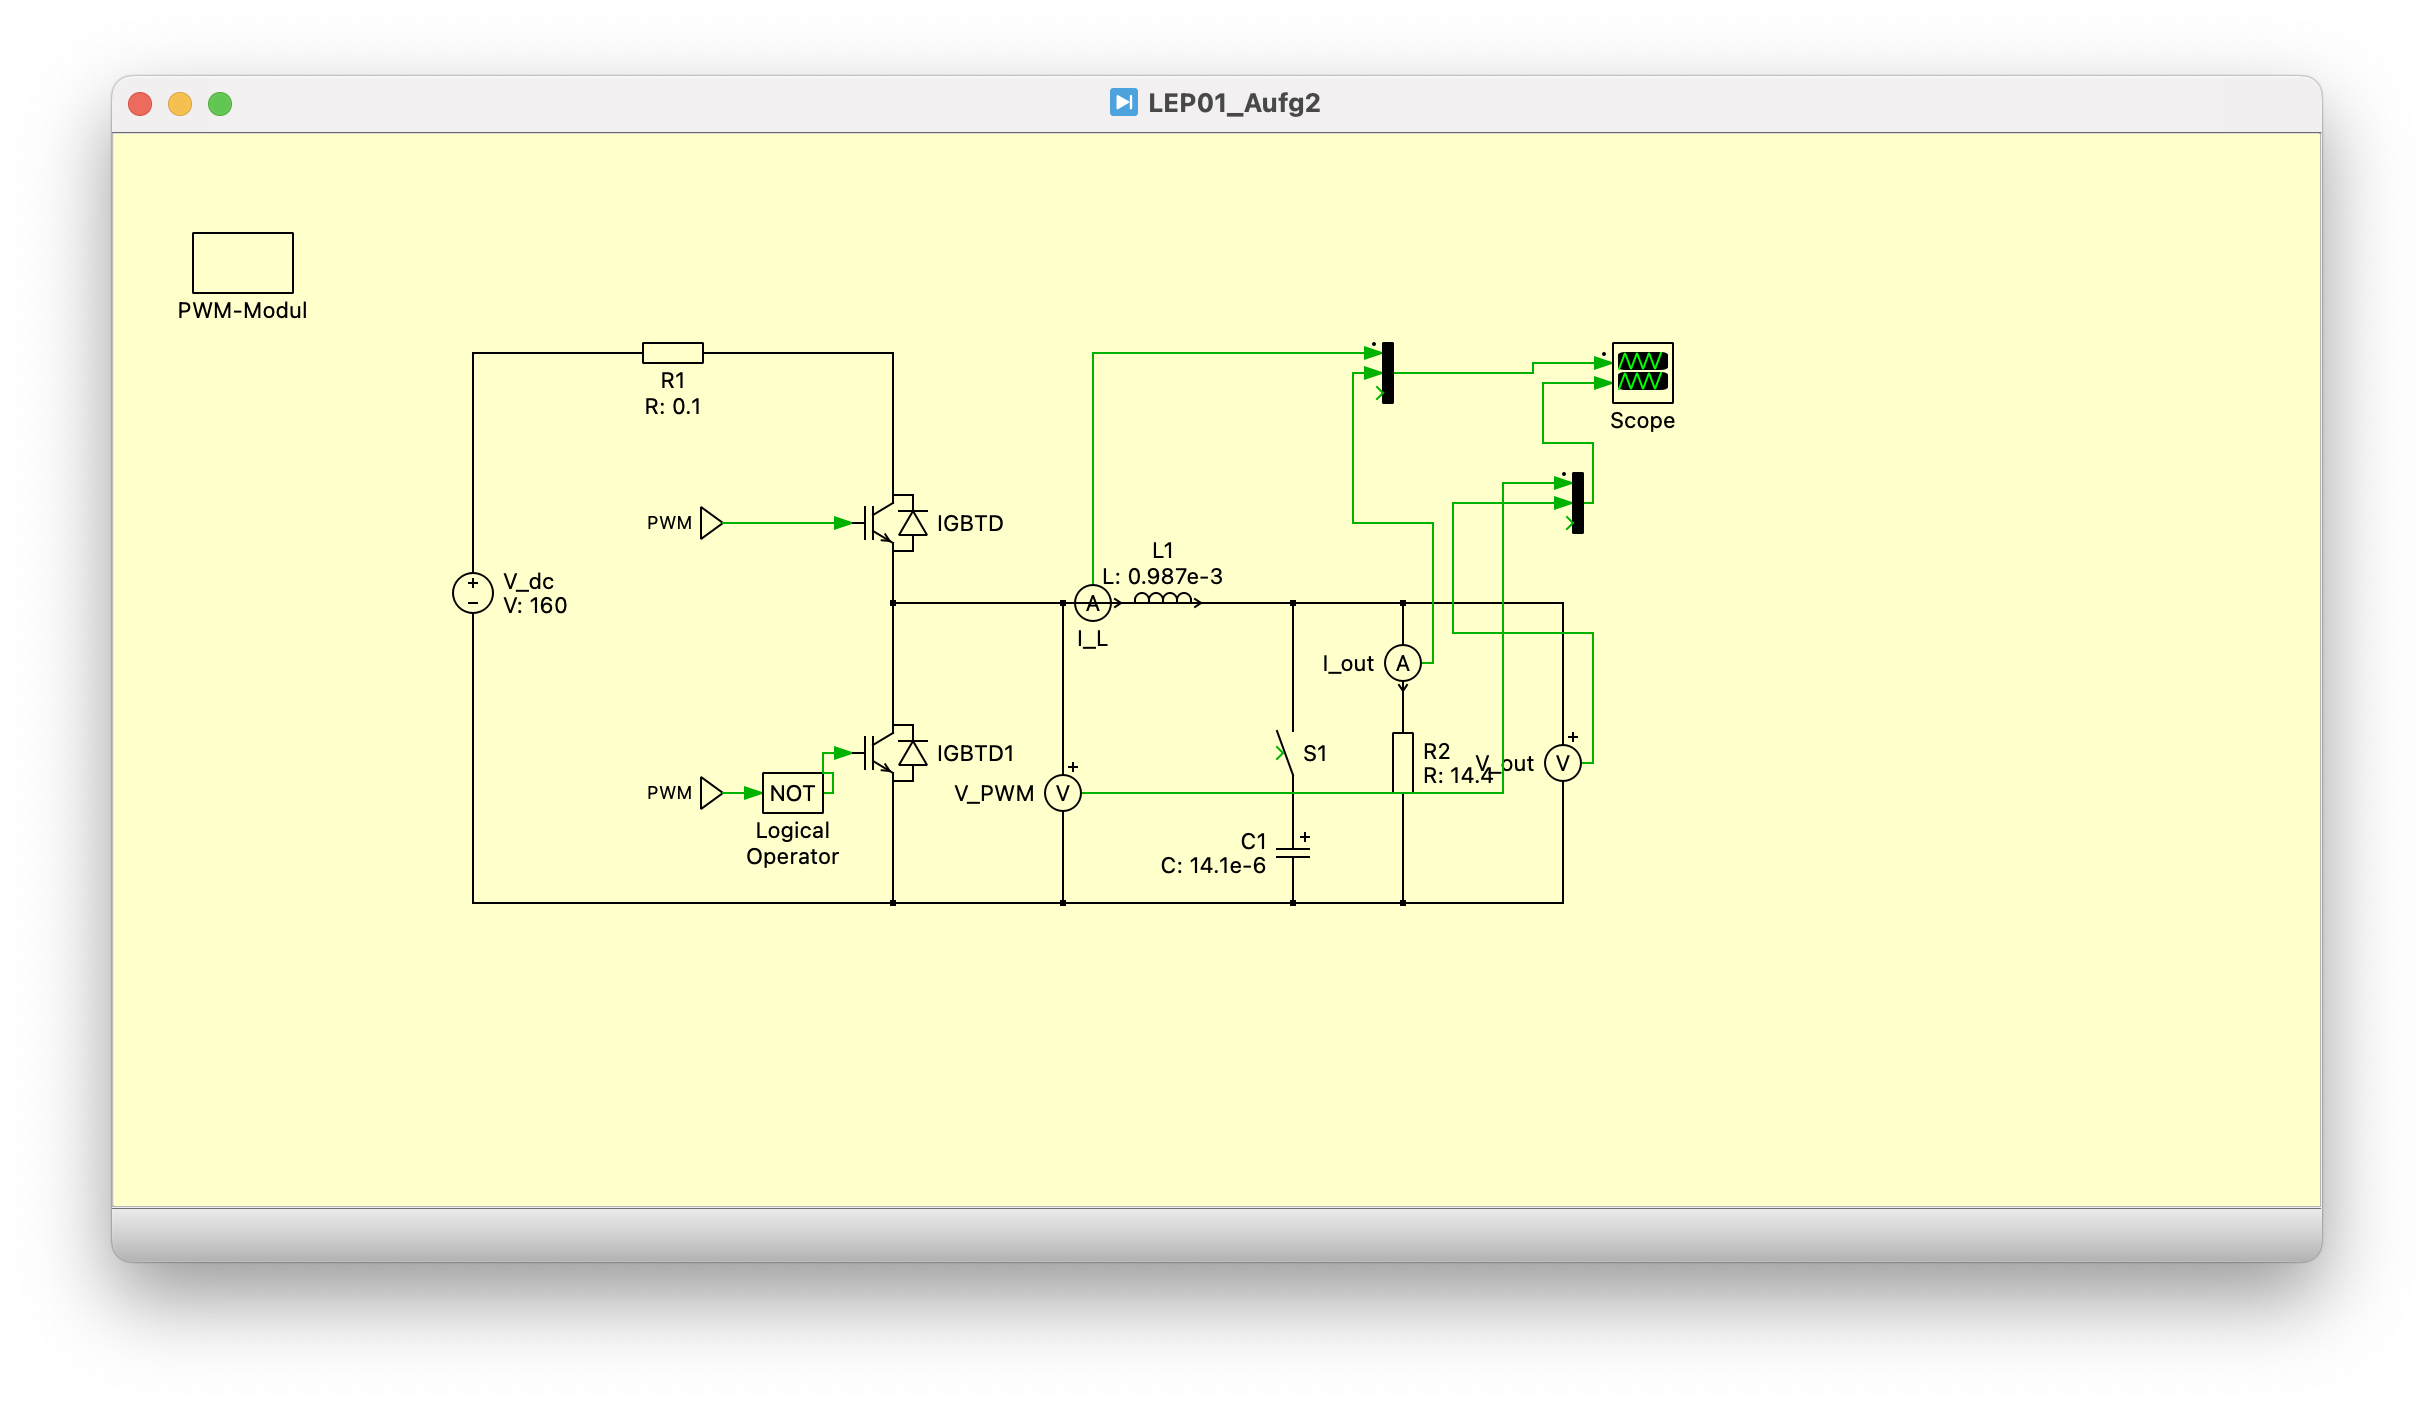
\includegraphics[width=0.95\textwidth]{assets/img/aufg2_aufbau.png}
  \end{center}
  \caption{Aufbau der Tiefsetzsteller-Schaltung für die zweite Aufgabe}
  \label{fig:aufg2_aufbau}
\end{figure}

Hier wird das PWM-Signal über ein GOTO-Block an die beiden IGBTs gegeben. Dabei wird ein Signal nicht-invertierend und das andere invertierend auf die Schaltung gegeben. Im Folgenden werden die Ein- und Ausgänge als Traces mit und ohne Kondensator betrachtet. Die Bauteile sind genau so dimensioniert wie in der ersten Aufgabe.

\begin{figure}[h]
  \begin{center}
    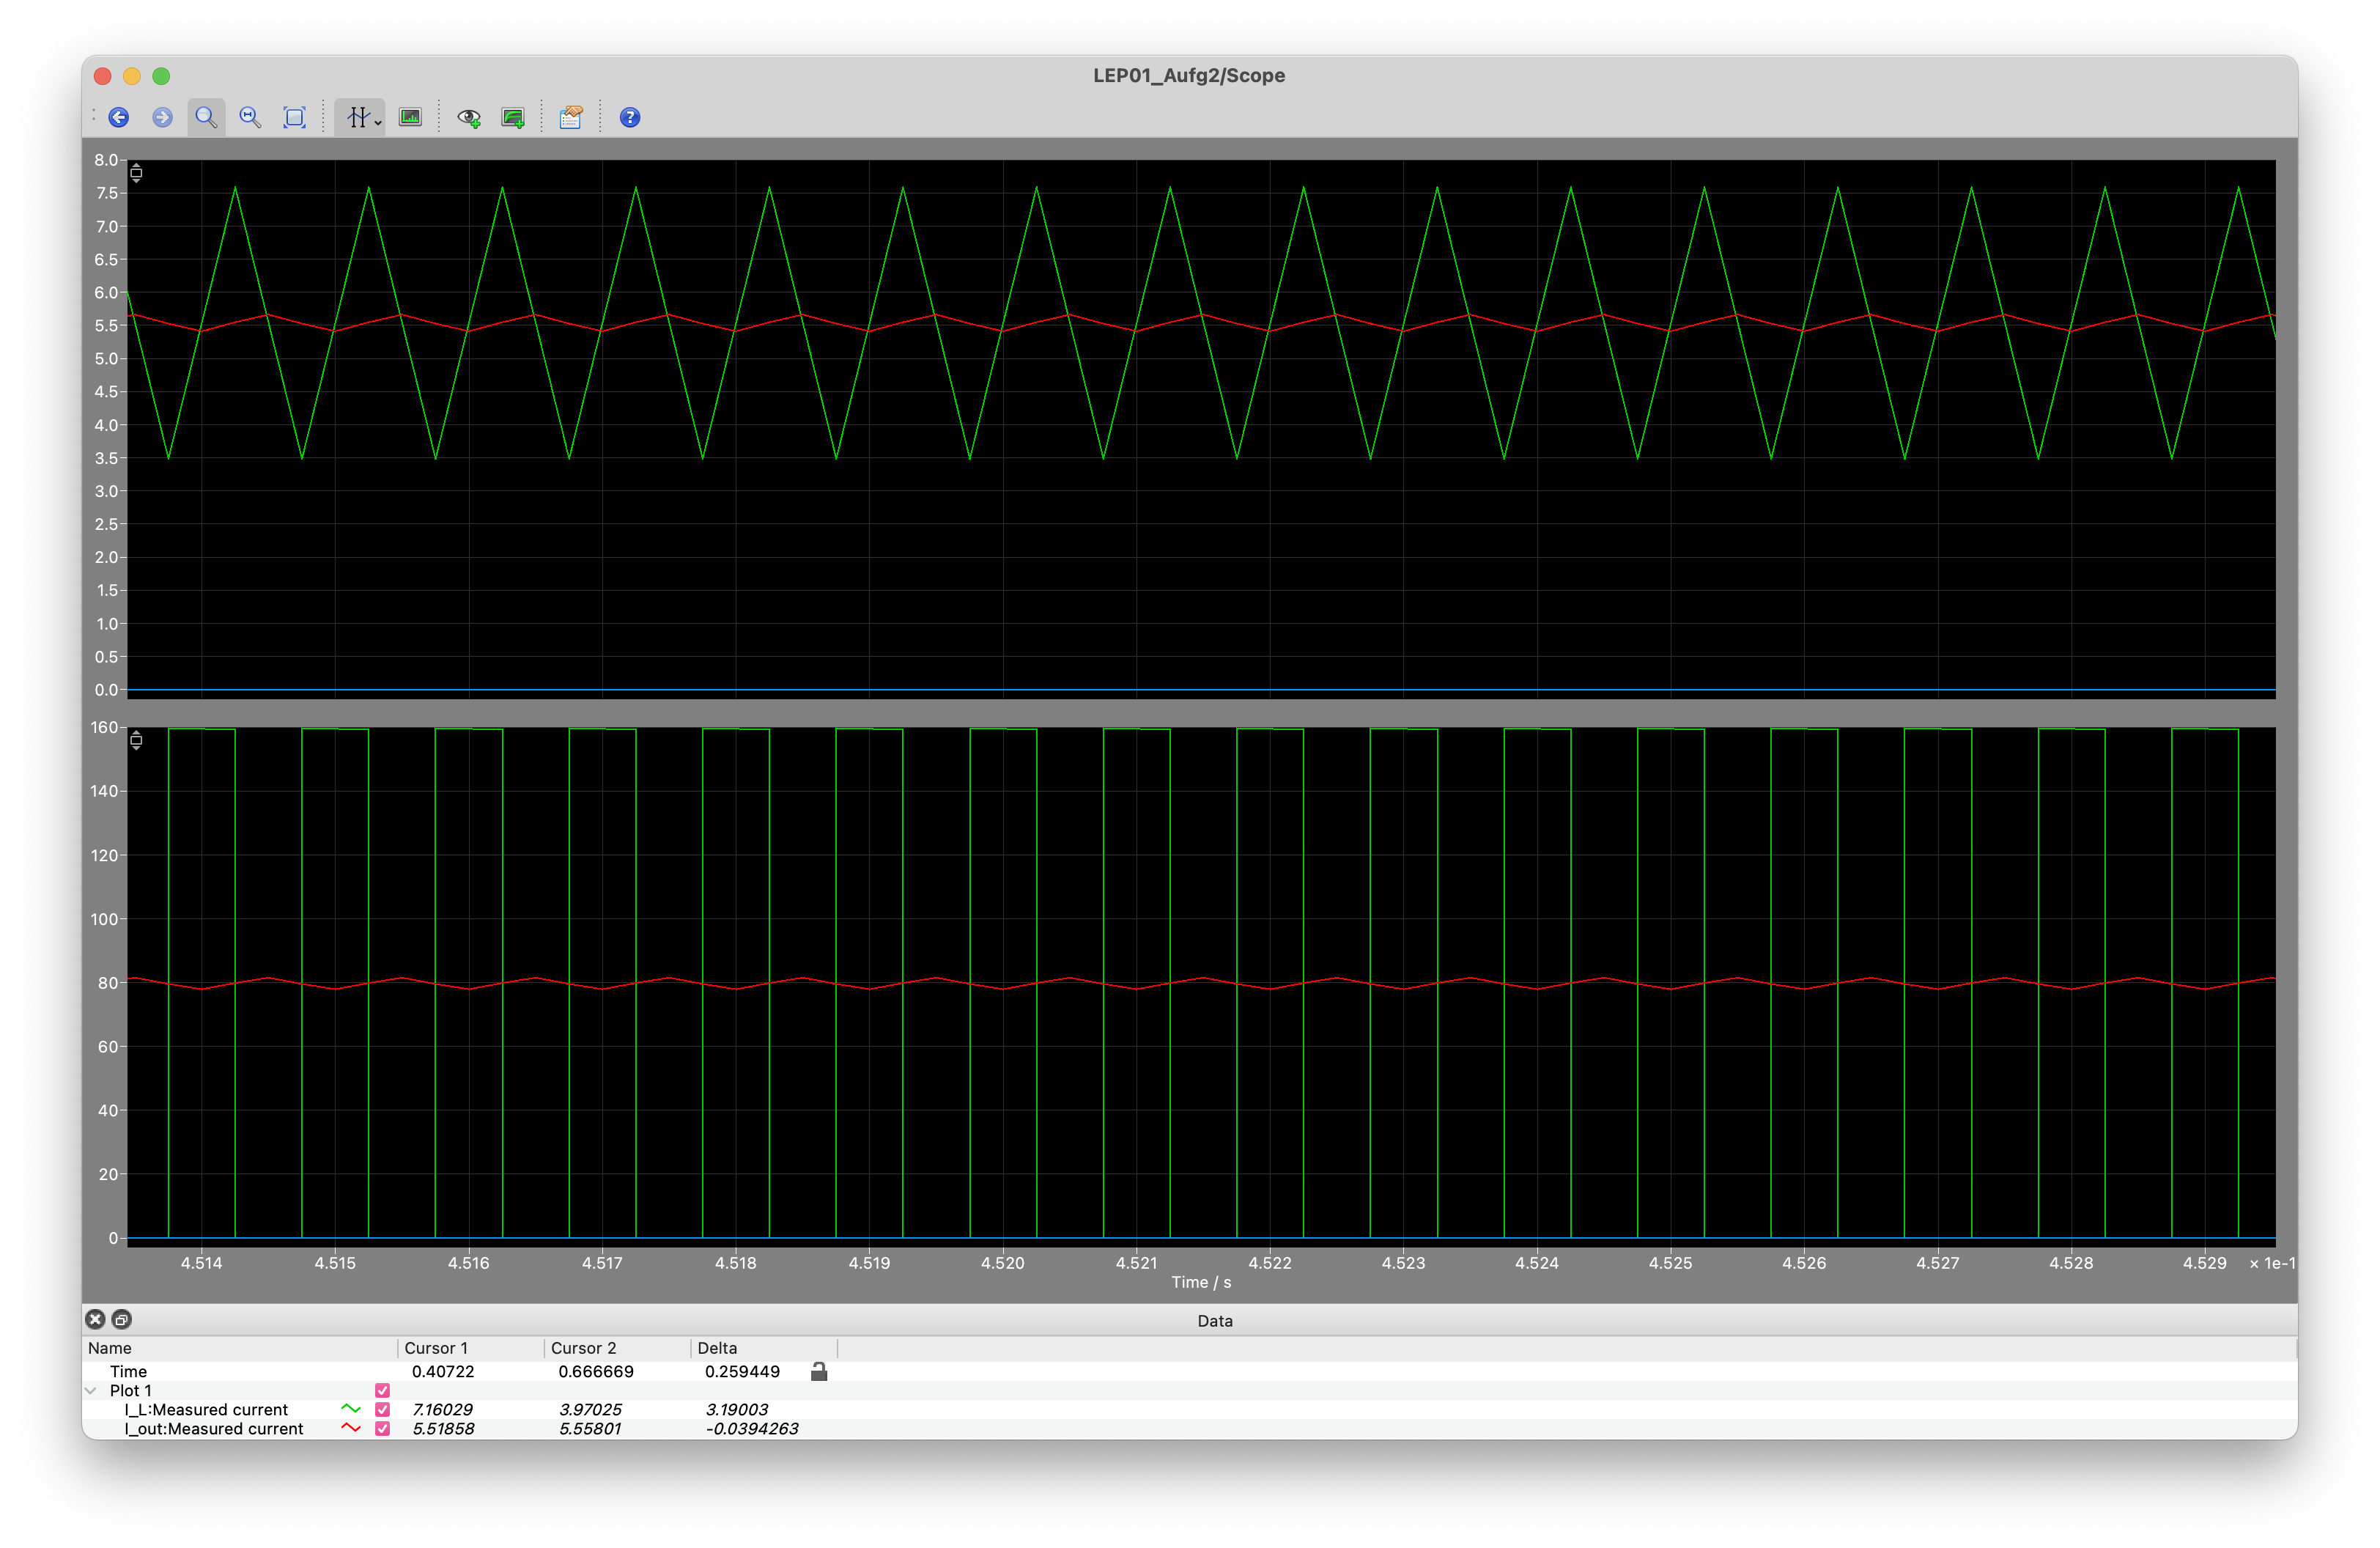
\includegraphics[width=0.95\textwidth]{assets/img/aufg2_eingang_ausgang_c_wc.png}
  \end{center}
  \caption{Die Ein- und Ausgänge der Schaltung im Betrieb mit Kondensator und konstantem PWM}
  \label{fig:aufg2_eingang_ausgang_c_wc}
\end{figure}

In Abbildung~\ref{fig:aufg2_eingang_ausgang_c_wc} ist der Betrieb gezeigt, der am nächsten an Aufgabe 1 dran ist. Mit einem konstanten PWM und einem Duty-Cycle von 0.5 sehen die Verläufe von Strom und Spannung am ähnlichsten zu Aufgabe 1 aus. 

\begin{figure}[h]
  \begin{center}
    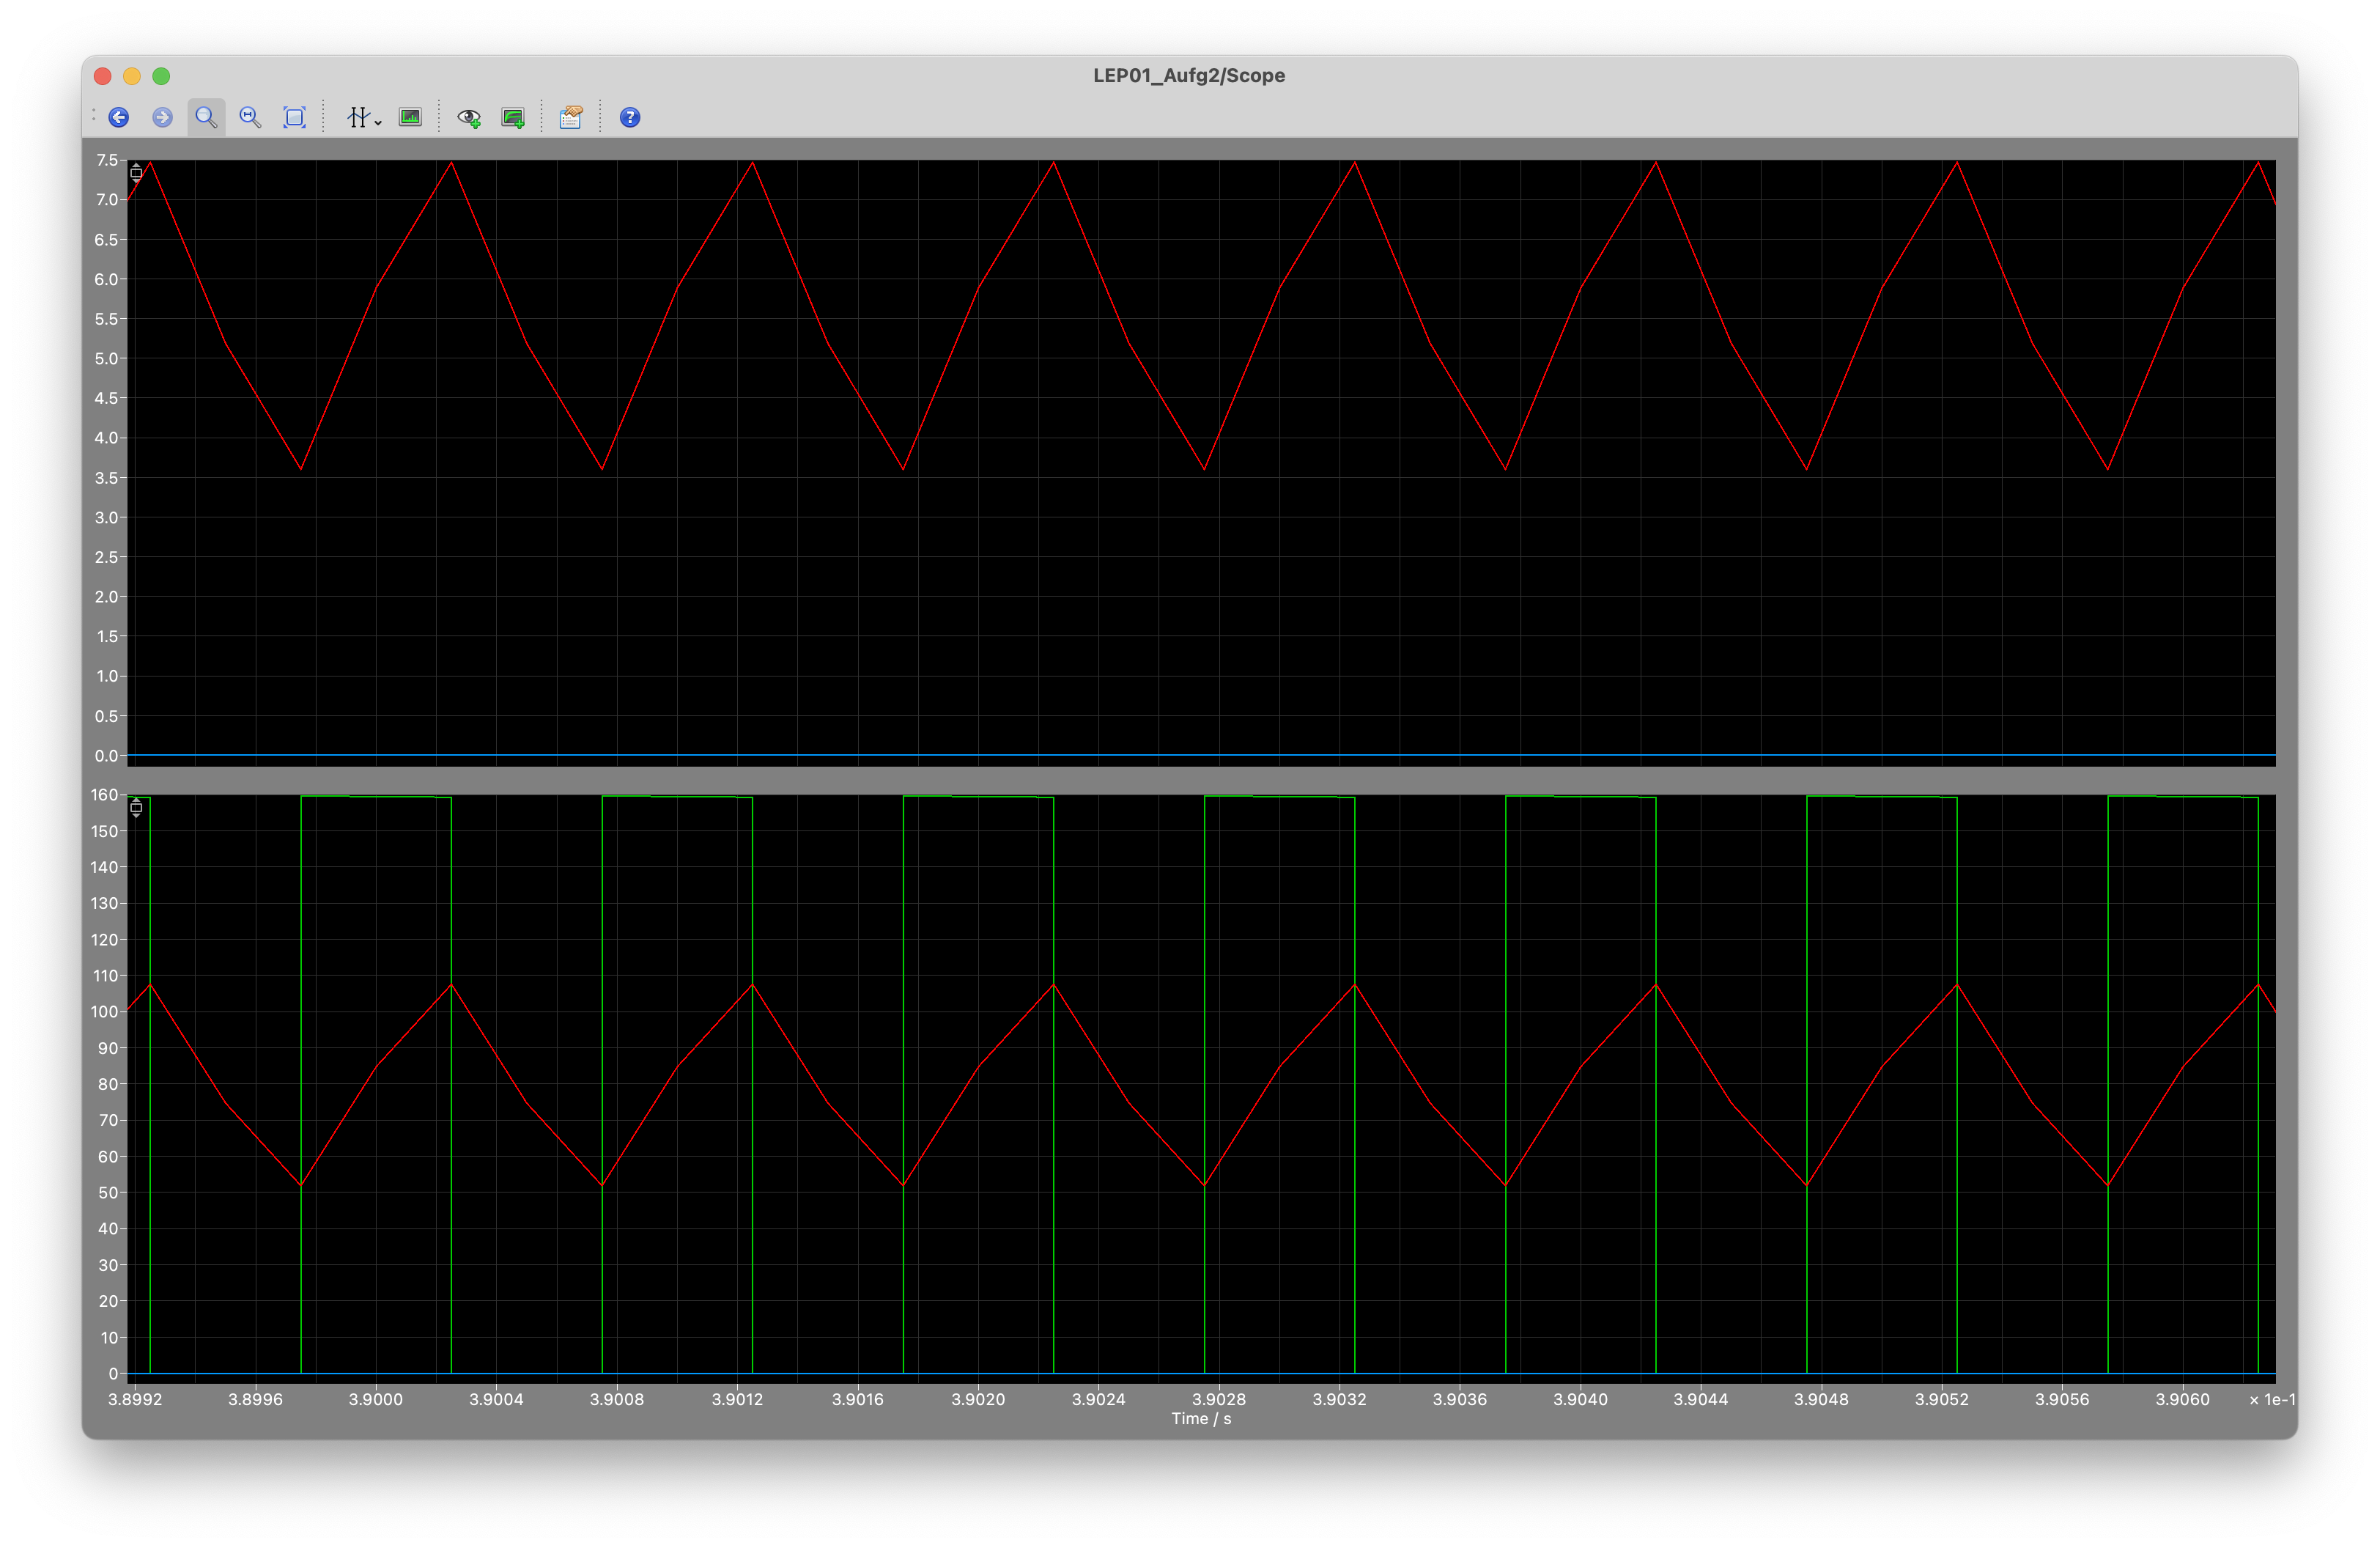
\includegraphics[width=0.95\textwidth]{assets/img/aufg2_eingang_ausgang_c_nc.png}
  \end{center}
  \caption{Die Ein- und Ausgänge der Schaltung im Betrieb ohne Kondensator und mit konstantem PWM}
  \label{fig:aufg2_eingang_ausgang_c_nc}
\end{figure}

Die Abbildung~\ref{fig:aufg2_eingang_ausgang_c_nc} ist zu sehen, dass der Strom durch die Spule und durch den Ausgangswiderstand identisch sind. Das liegt daran, dass nun die Verbindung zum Kondensator offen ist und deshalb Spule und Ausganswiderstand in einer Masche liegen. Darüber hinaus ist deutlich zu erkennen, dass dadurch der Strom durch den Ausgangswiderstand deutlich stärker schwingt, da er nicht mehr durch den Kondensator geglättet wird. 

\begin{figure}[h]
  \begin{center}
    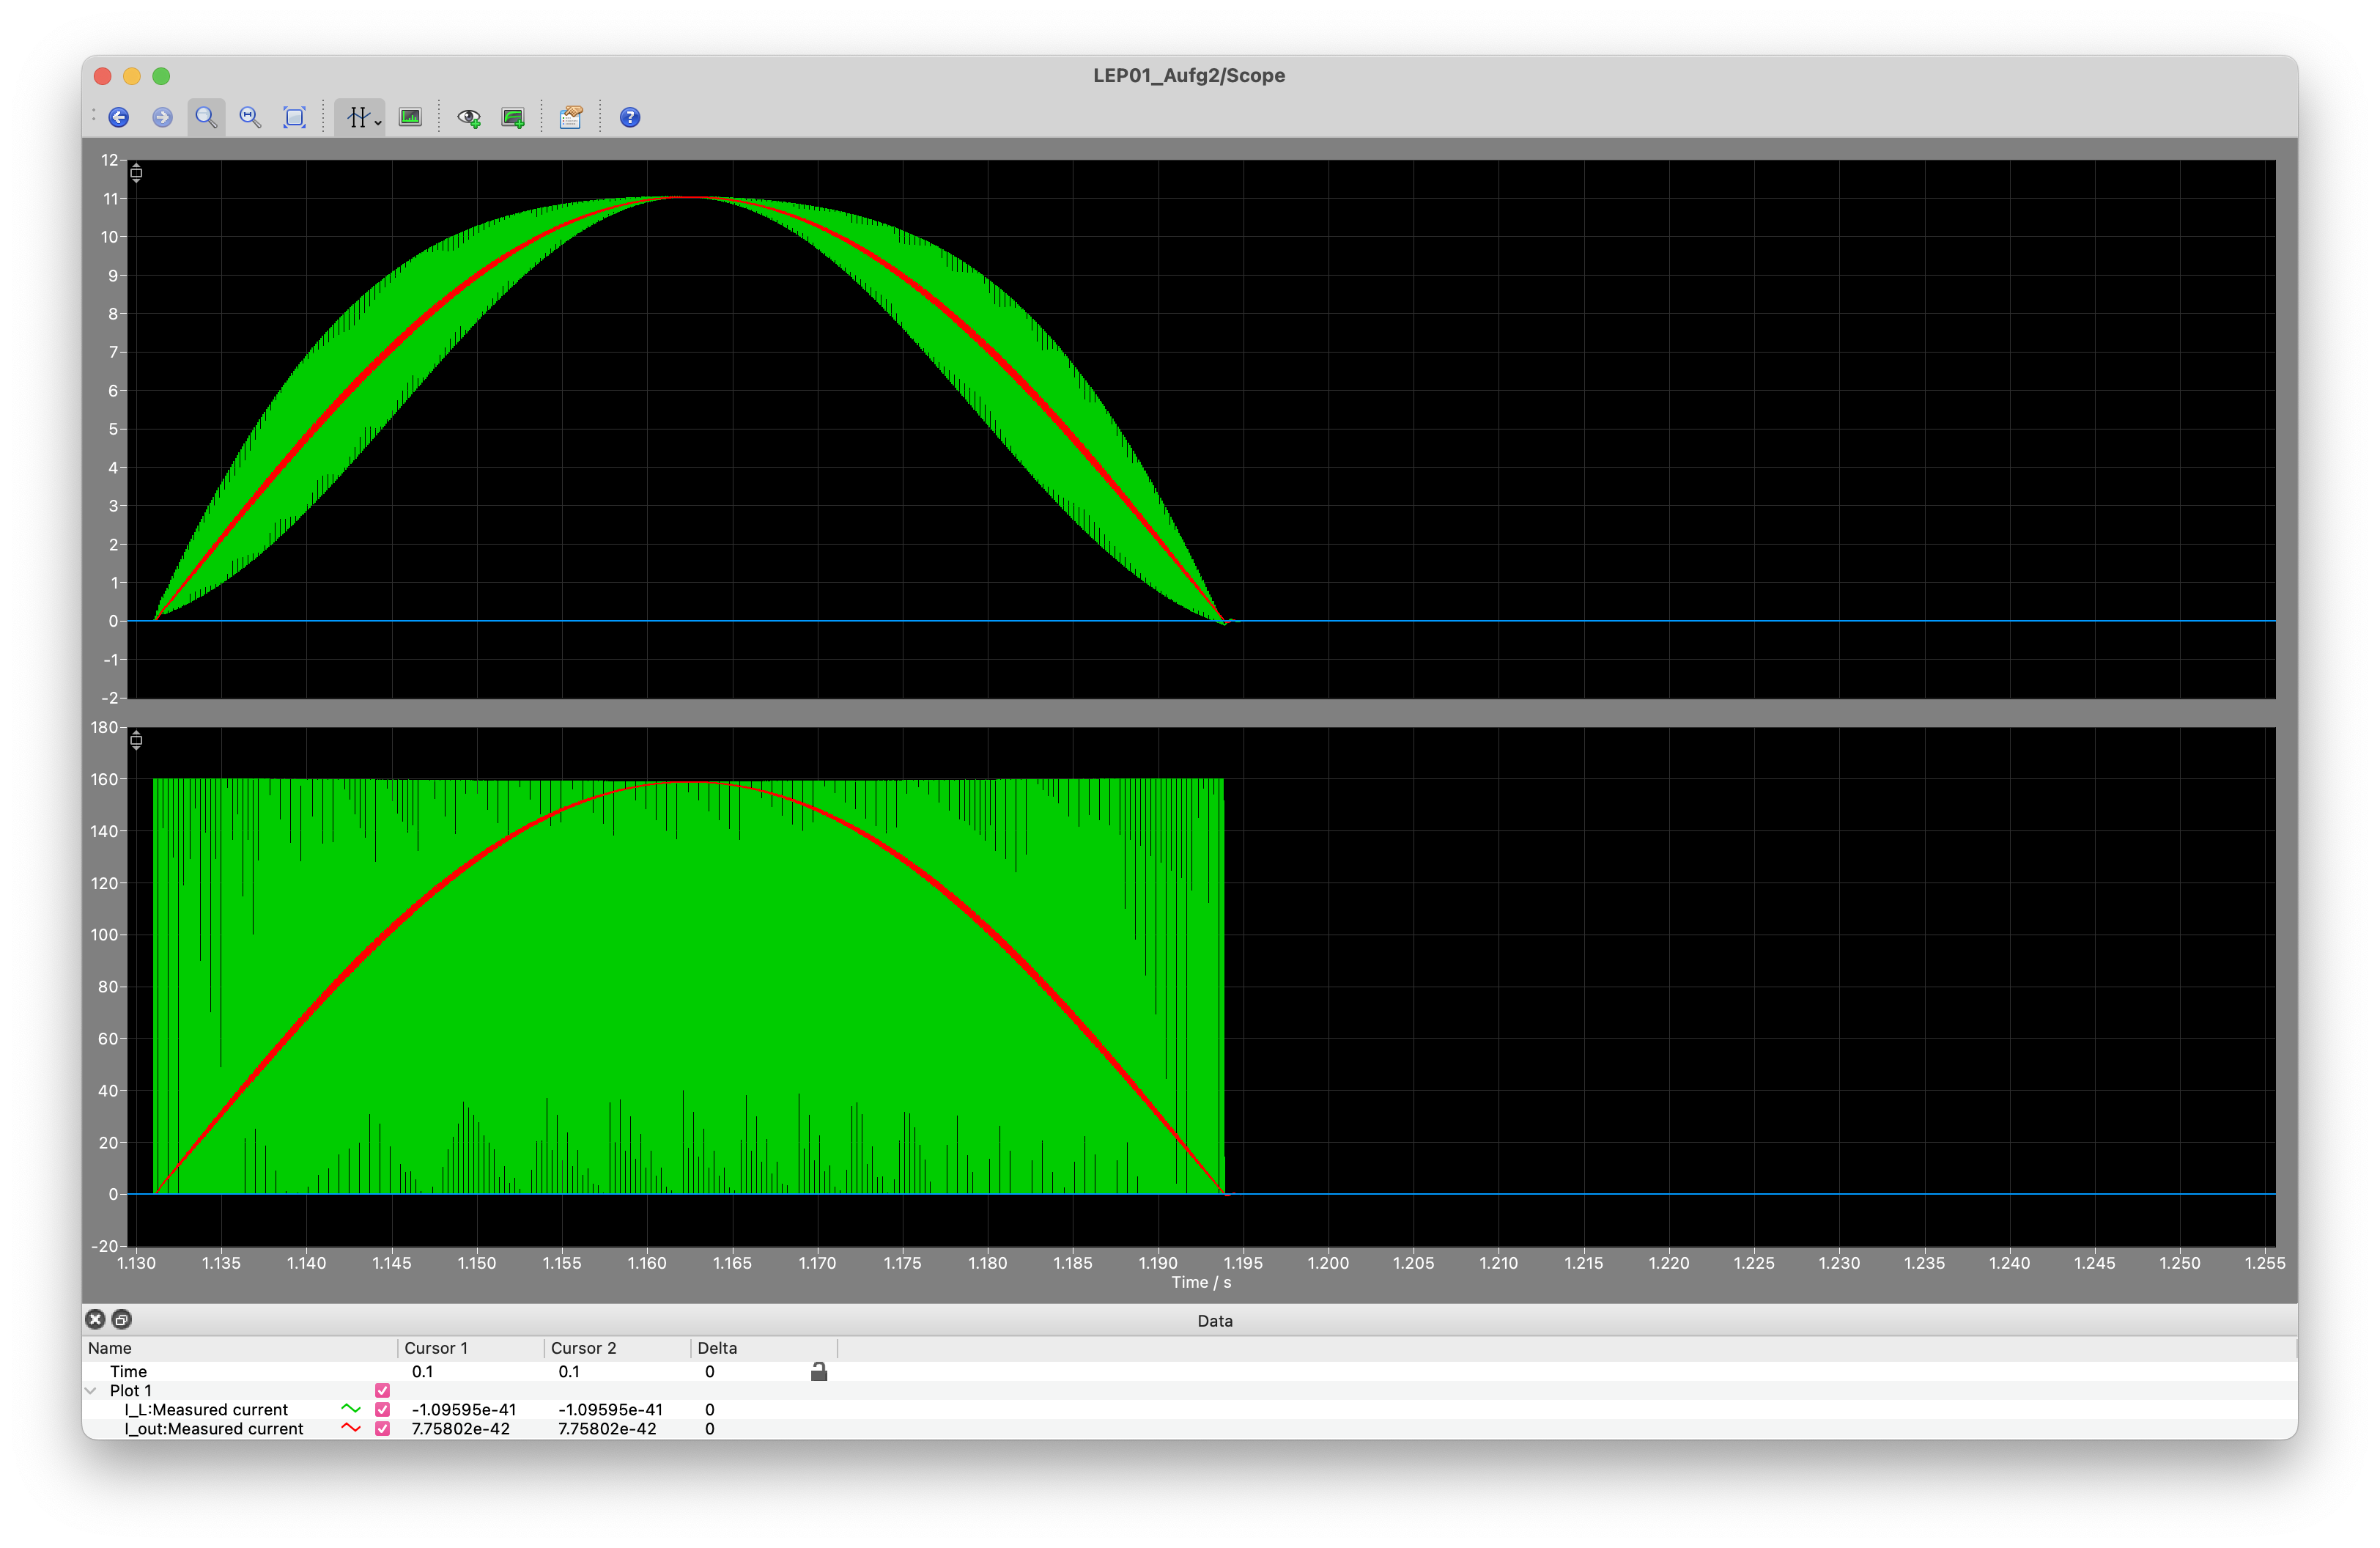
\includegraphics[width=0.95\textwidth]{assets/img/aufg2_eingang_ausgang_sin_wc.png}
  \end{center}
  \caption{Die Ein- und Ausgänge der Schaltung im Betrieb mit Kondensator und Sinus-Signal als PWM}
  \label{fig:aufg2_eingang_ausgang_sin_wc}
\end{figure}

Im Betrieb mit Kondensator und mit Sinus-PWM-Signal, wie in Abbildung~\ref{fig:aufg2_eingang_ausgang_sin_wc} zu sehen ist, steigt der Strom und die Spannung, die die Schaltung auf den Ausgangswiderstand gibt mit steigendem Sinussignal proportional an. Sobald die Sinuswelle im Negativen ist, ist das Bauteil unbelastet, da hier auch kein PWM-Signal durch die PWM-Schaltung bereitgestellt wird. 

\begin{figure}[h]
  \begin{center}
    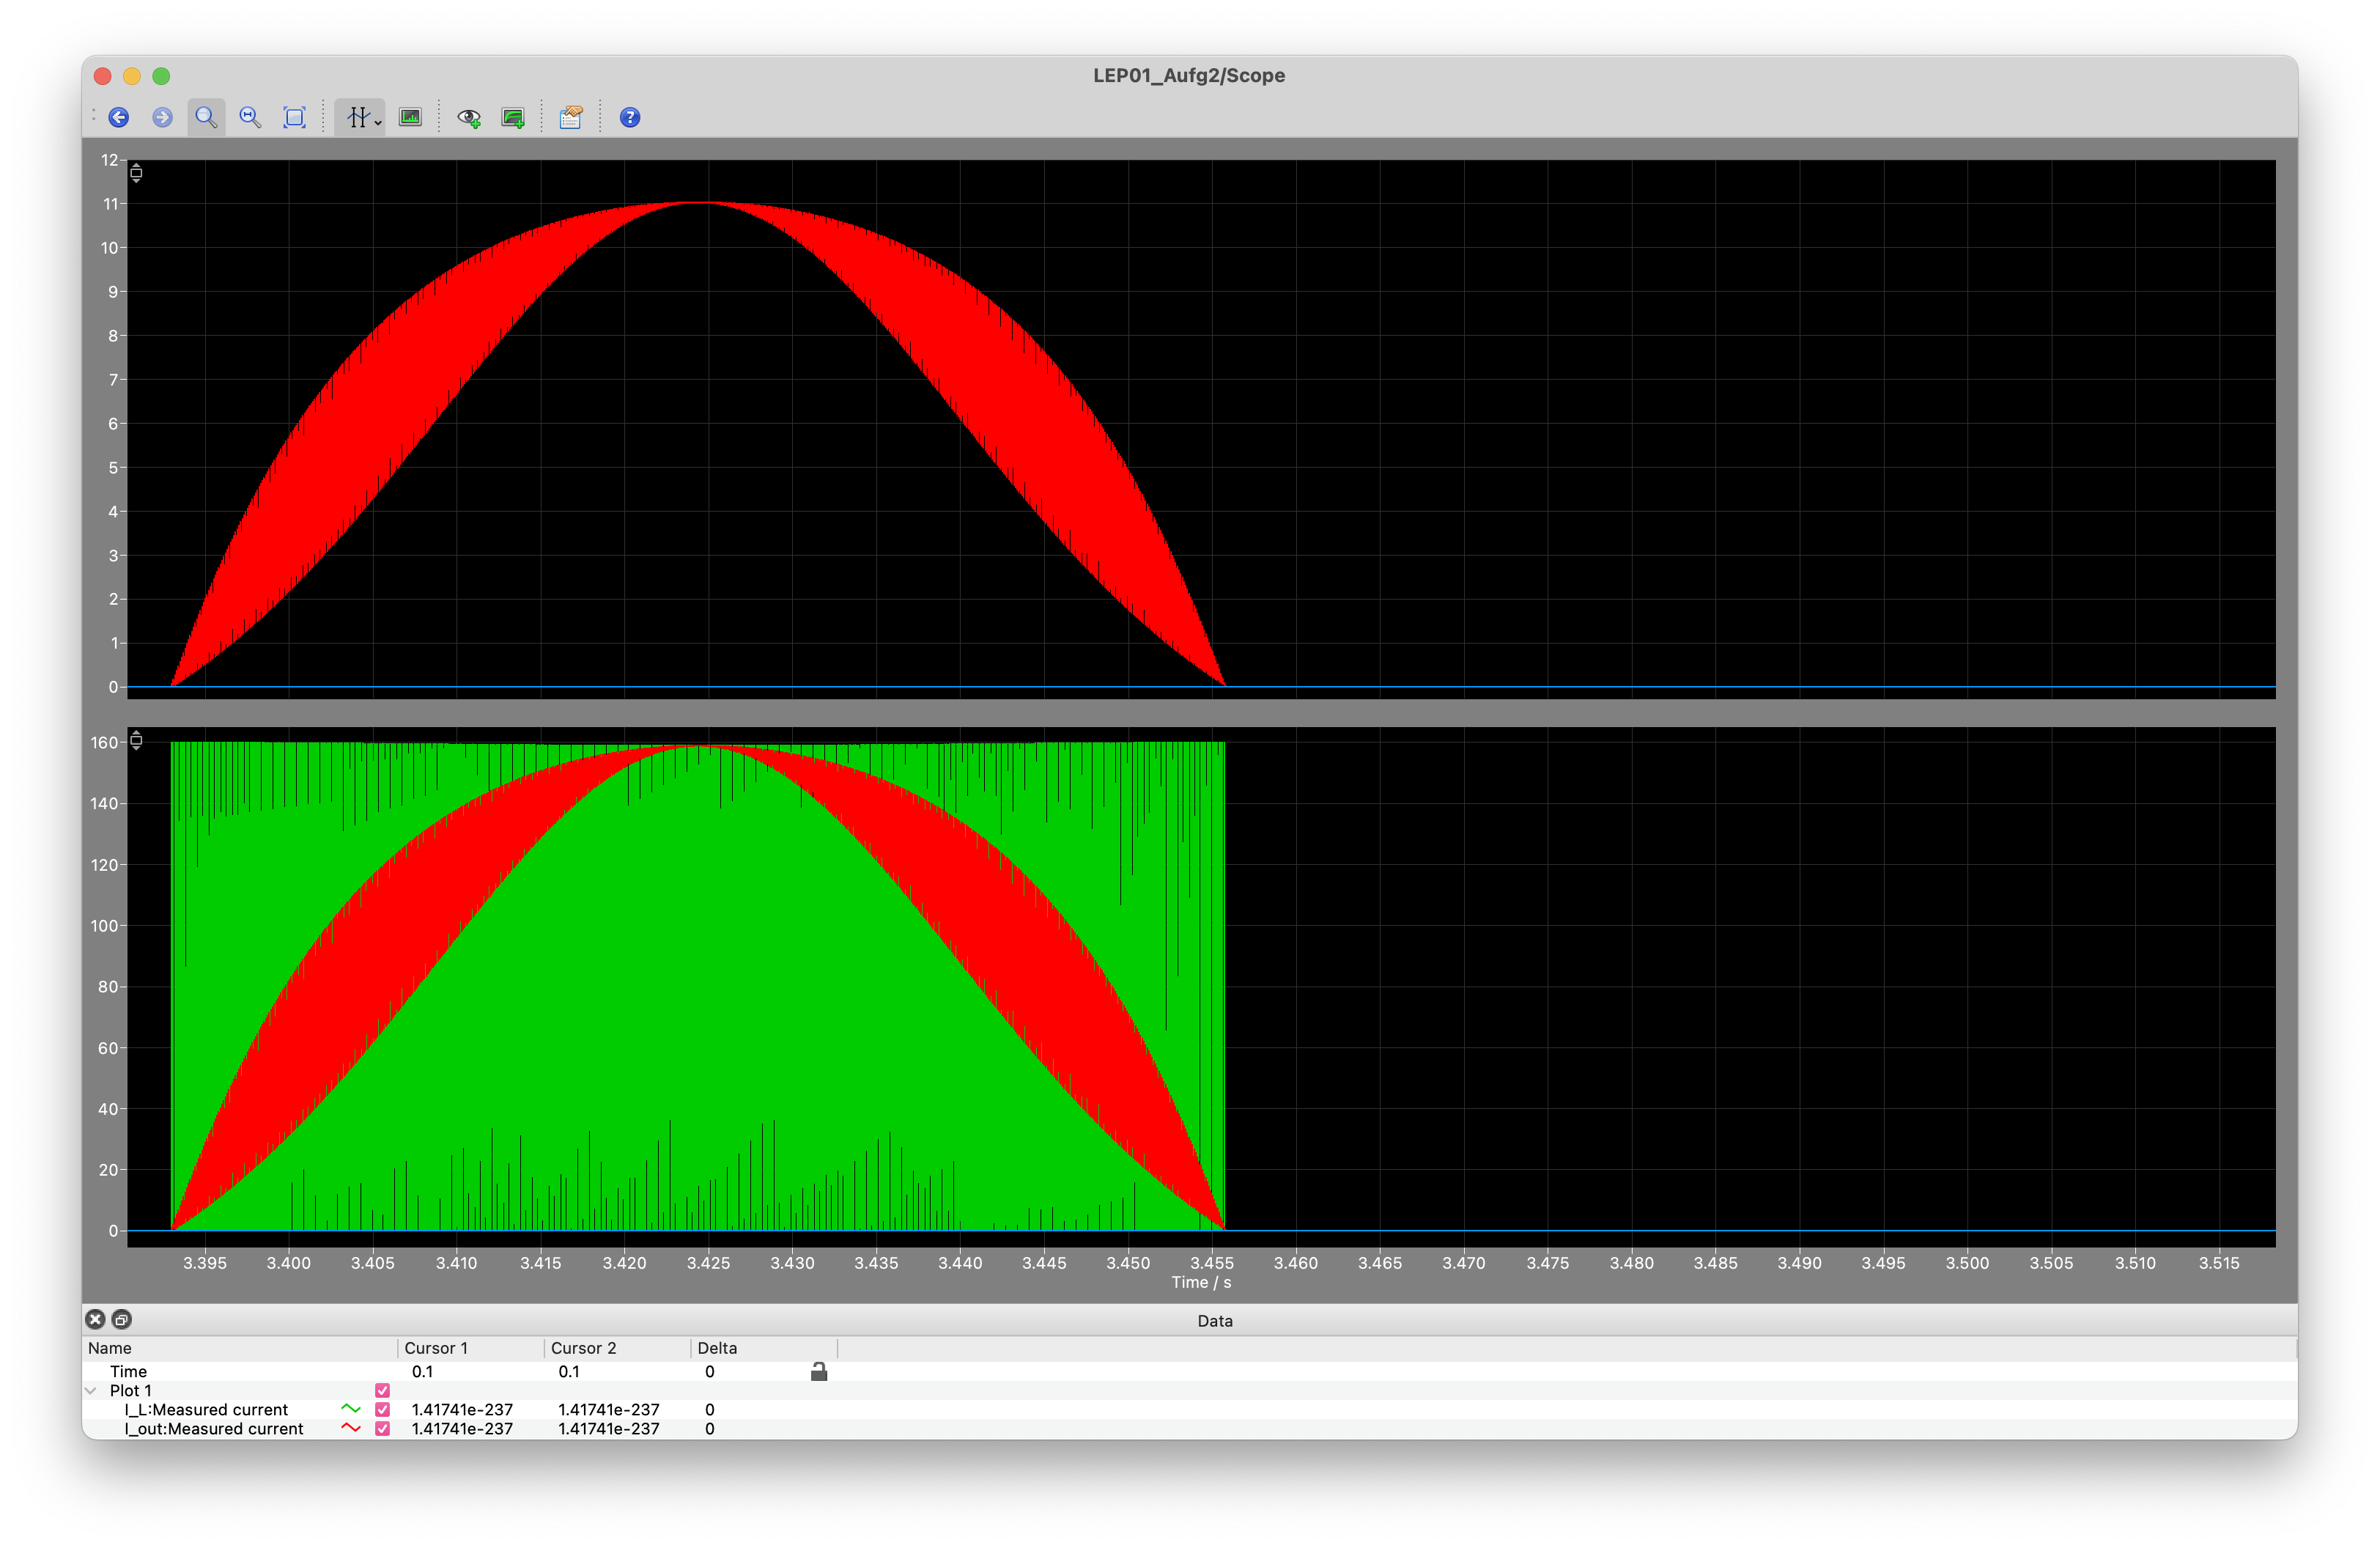
\includegraphics[width=0.95\textwidth]{assets/img/aufg2_eingang_ausgang_sin_nc.png}
  \end{center}
  \caption{Die Ein- und Ausgänge der Schaltung im Betrieb ohne Kondensator und Sinus-Signal als PWM}
  \label{fig:aufg2_eingang_ausgang_sin_nc}
\end{figure}


\end{document}
